%%%%%%%%%%%%%%%%%%%%%%%%%%%%%%%%%%%%%%%%%%%%%%%%%%%%%%%%%%%%%%%%%%%%%%%%%%%%%%%%%%
\begin{frame}[fragile]\frametitle{}
\begin{center}
{\Large Introduction to Graphs}
\end{center}
\end{frame}



%%%%%%%%%%%%%%%%%%%%%%%%%%%%%%%%%%%%%%%%%%%%%%%%%%%%%%%%%%%%%%%%%%%%%%%%%%%%%%%%%%
\begin{frame}\frametitle{A graph is}
{\emph \ldots a set of discrete objects, each of which has some set of relationships with the other objects}

Euler: Can we take a walk to all 4 islands, without crossing any of the bridge twice?

Abstraction (Does size of islands matter?):

\begin{center}
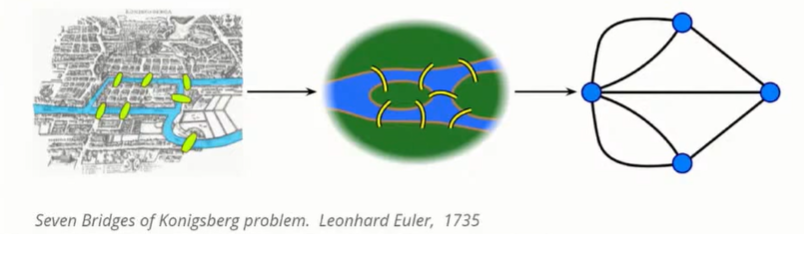
\includegraphics[width=\linewidth,keepaspectratio]{neo4j4}
\end{center}	  

Solution: No way!! What's the rule?

{\tiny (Ref: Introduction to Neo4j - a hands-on crash course - neo4j)}
\end{frame}


%%%%%%%%%%%%%%%%%%%%%%%%%%%%%%%%%%%%%%%%%%%%%%%%%%%%%%%%%%%
\begin{frame}[fragile]\frametitle{ Graph-structured Data Are Ubiquitous }

\begin{center}
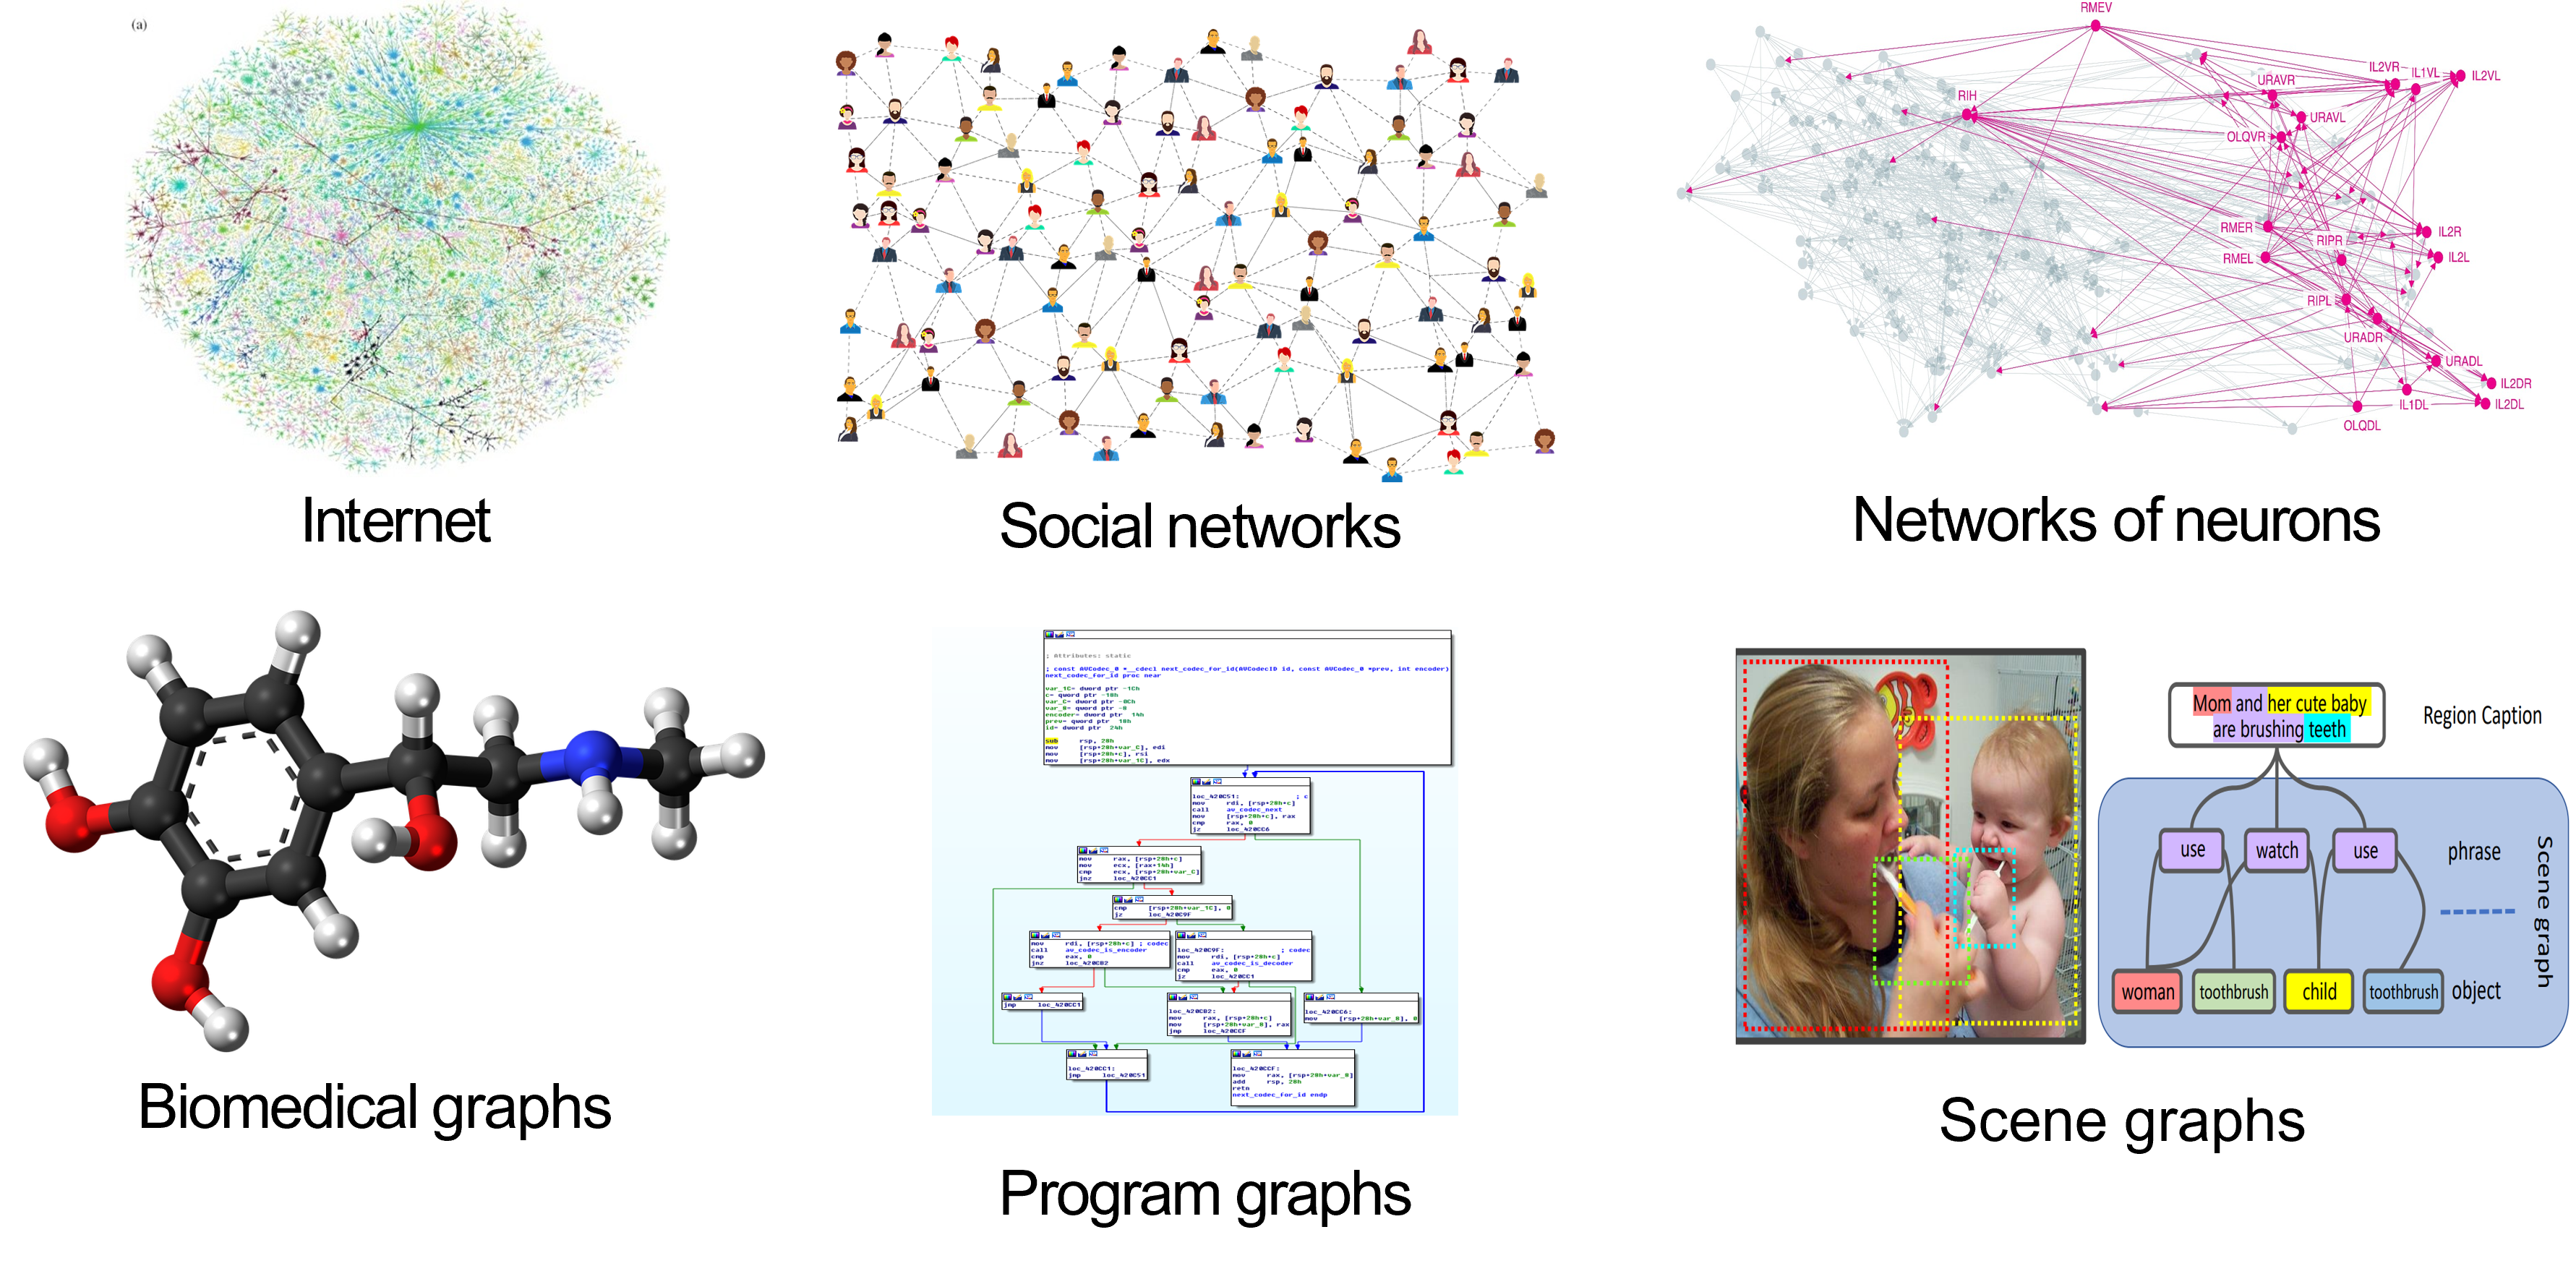
\includegraphics[width=\linewidth,keepaspectratio]{gnn1}
\end{center}	  

\end{frame}

%%%%%%%%%%%%%%%%%%%%%%%%%%%%%%%%%%%%%%%%%%%%%%%%%%%%%%%%%%%
\begin{frame}[fragile]\frametitle{}

\begin{center}
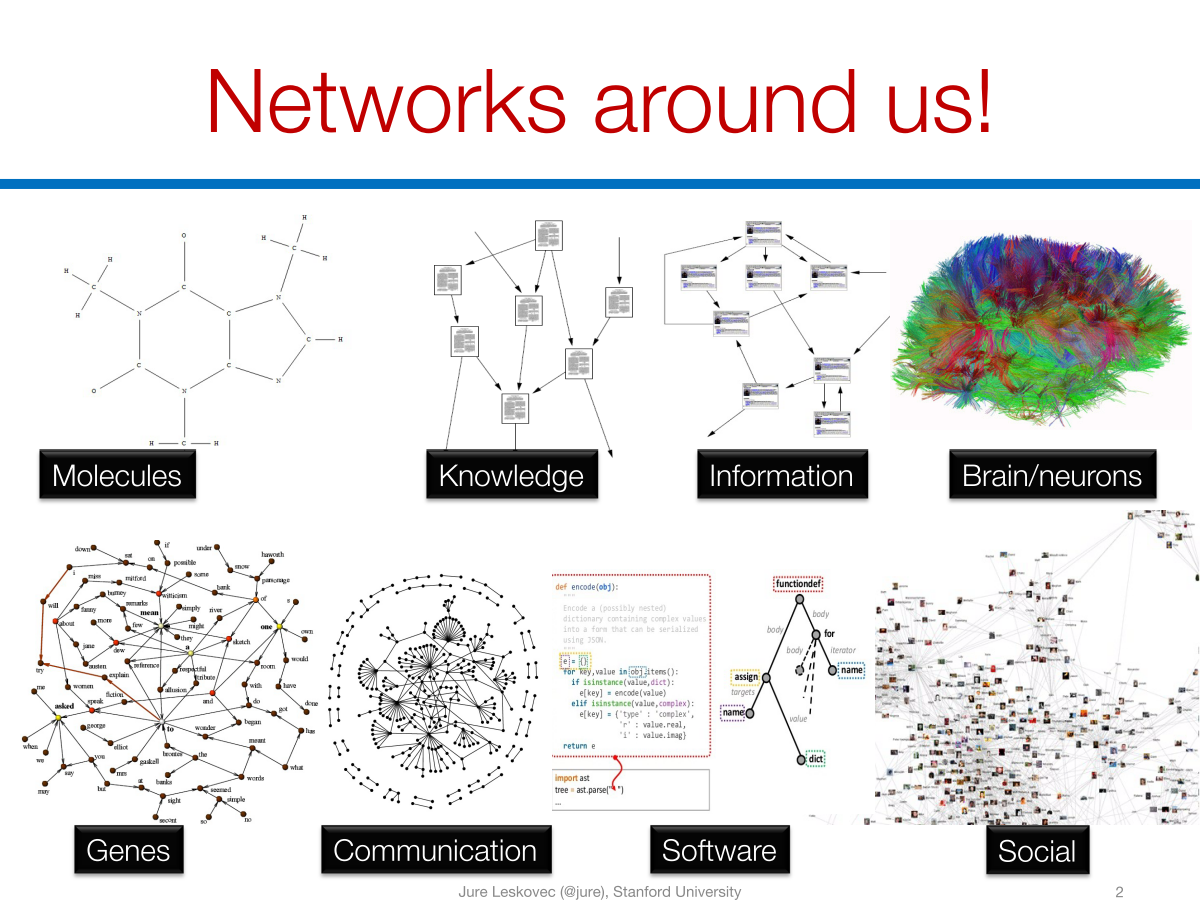
\includegraphics[width=\linewidth,keepaspectratio]{gnn2}
\end{center}	  

\end{frame}

%%%%%%%%%%%%%%%%%%%%%%%%%%%%%%%%%%%%%%%%%%%%%%%%%%%%%%%%%%%
\begin{frame}[fragile]\frametitle{}

\begin{center}
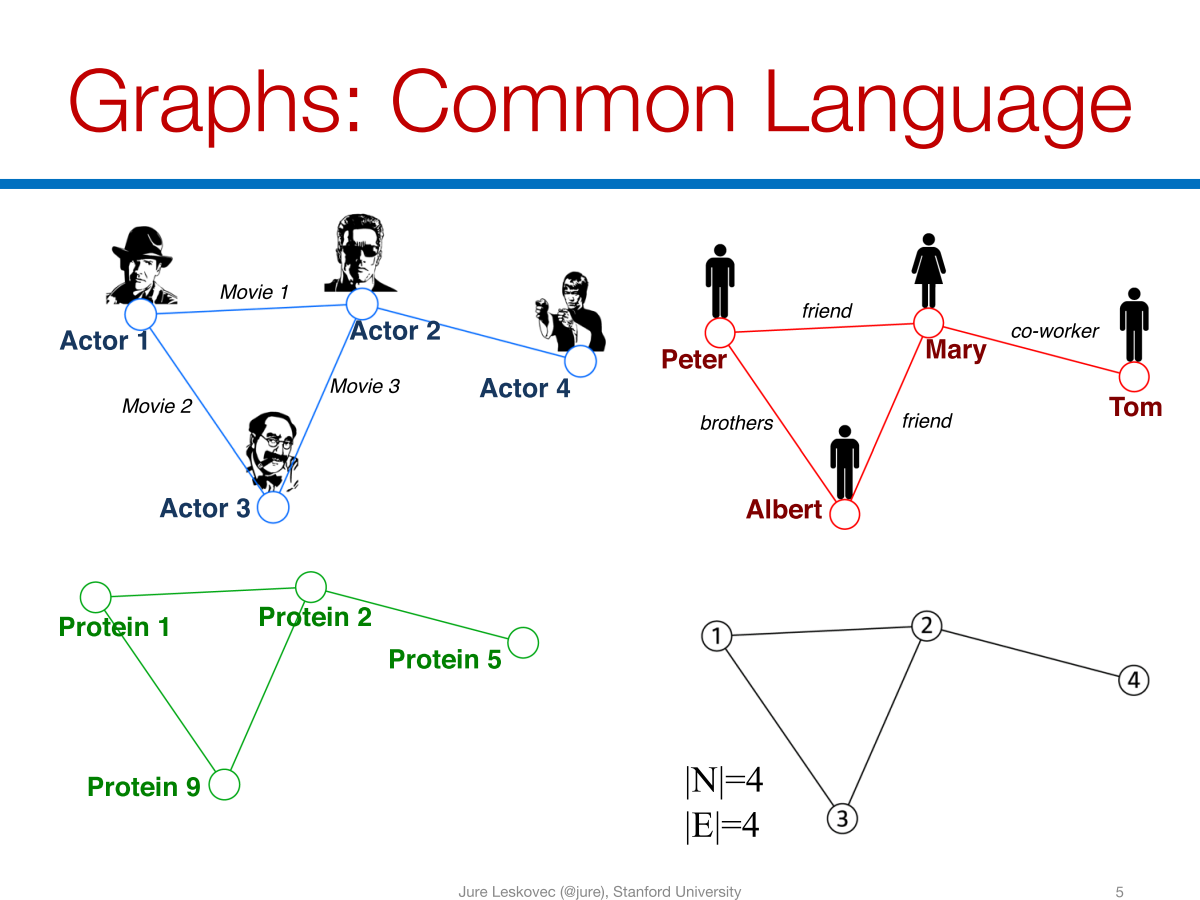
\includegraphics[width=\linewidth,keepaspectratio]{gnn3}
\end{center}	  

\end{frame}

%%%%%%%%%%%%%%%%%%%%%%%%%%%%%%%%%%%%%%%%%%%%%%%%%%%%%%%%%%%%%%%%%%%%%%%%%%%%%%%%%%
\begin{frame}\frametitle{ Why do graphs matter? }

Across an organization, every department can benefit from graphs to answer questions 
like who or what is important, what should I do next, and what’s unusual about this?

\begin{center}
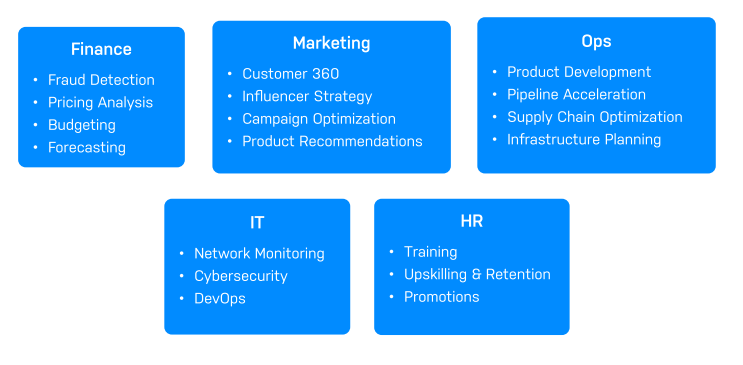
\includegraphics[width=\linewidth,keepaspectratio]{neo4j103}
\end{center}	  


{\tiny (Ref: 5 Graph Data Science Basics Everyone Should Know - neo4j)}
\end{frame}

%%%%%%%%%%%%%%%%%%%%%%%%%%%%%%%%%%%%%%%%%%%%%%%%%%%%%%%%%%%
\begin{frame}[fragile]\frametitle{Graphs: A Universal Language }

\begin{center}
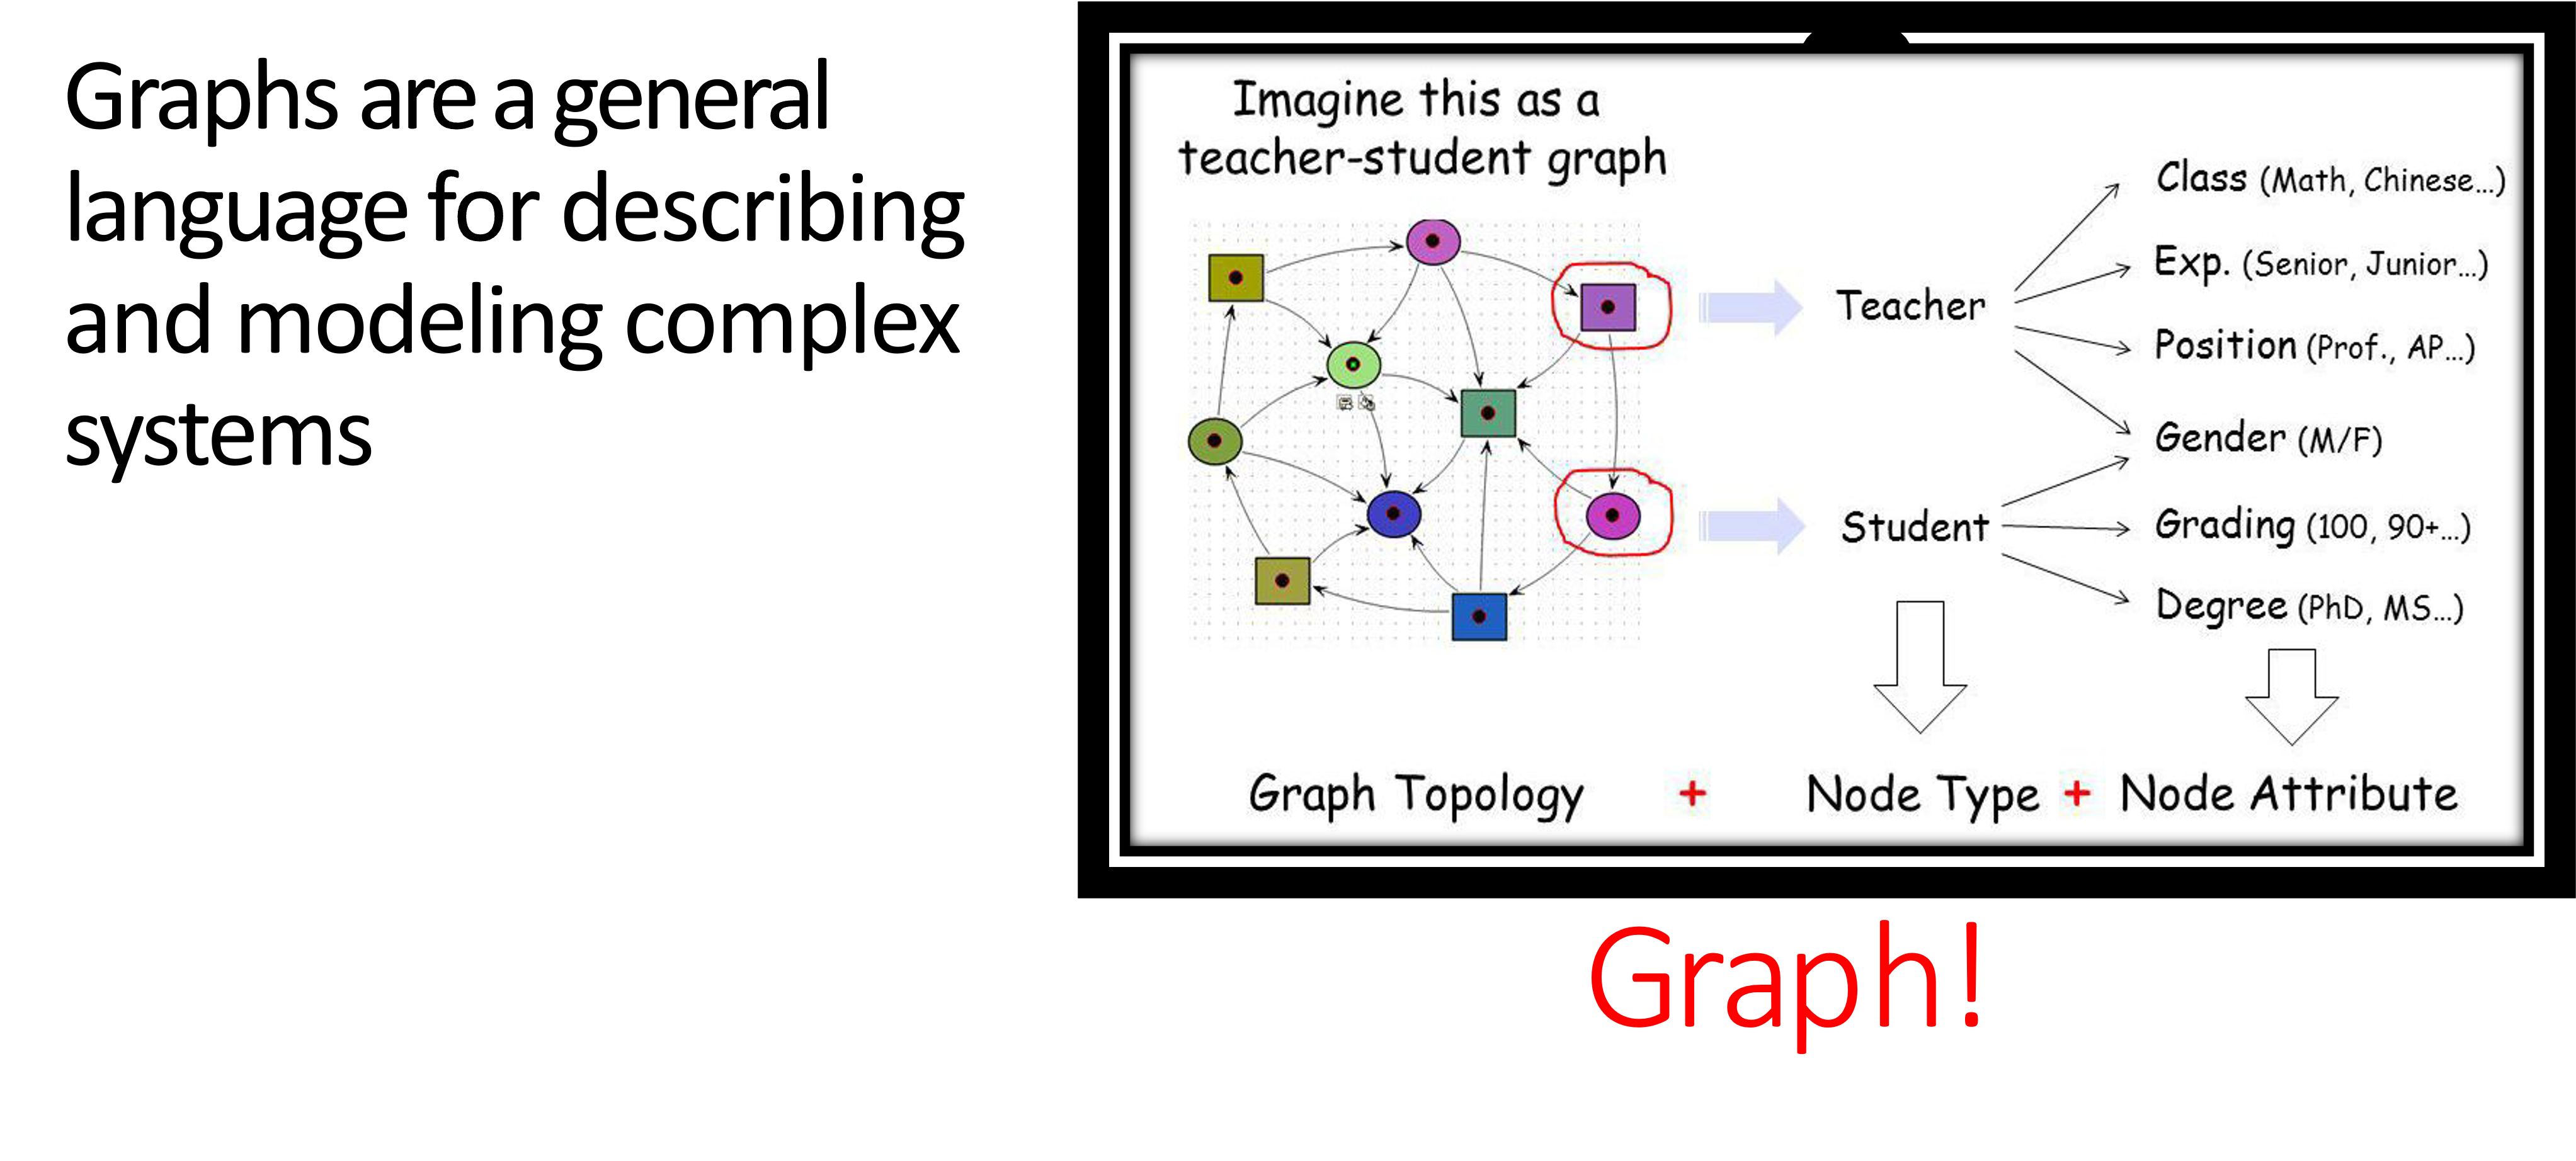
\includegraphics[width=\linewidth,keepaspectratio]{gnn4}
\end{center}	  

\end{frame}


%%%%%%%%%%%%%%%%%%%%%%%%%%%%%%%%%%%%%%%%%%%%%%%%%%%%%%%%%%%
\begin{frame}[fragile]\frametitle{Data as Graphs - Explicit }

\begin{center}
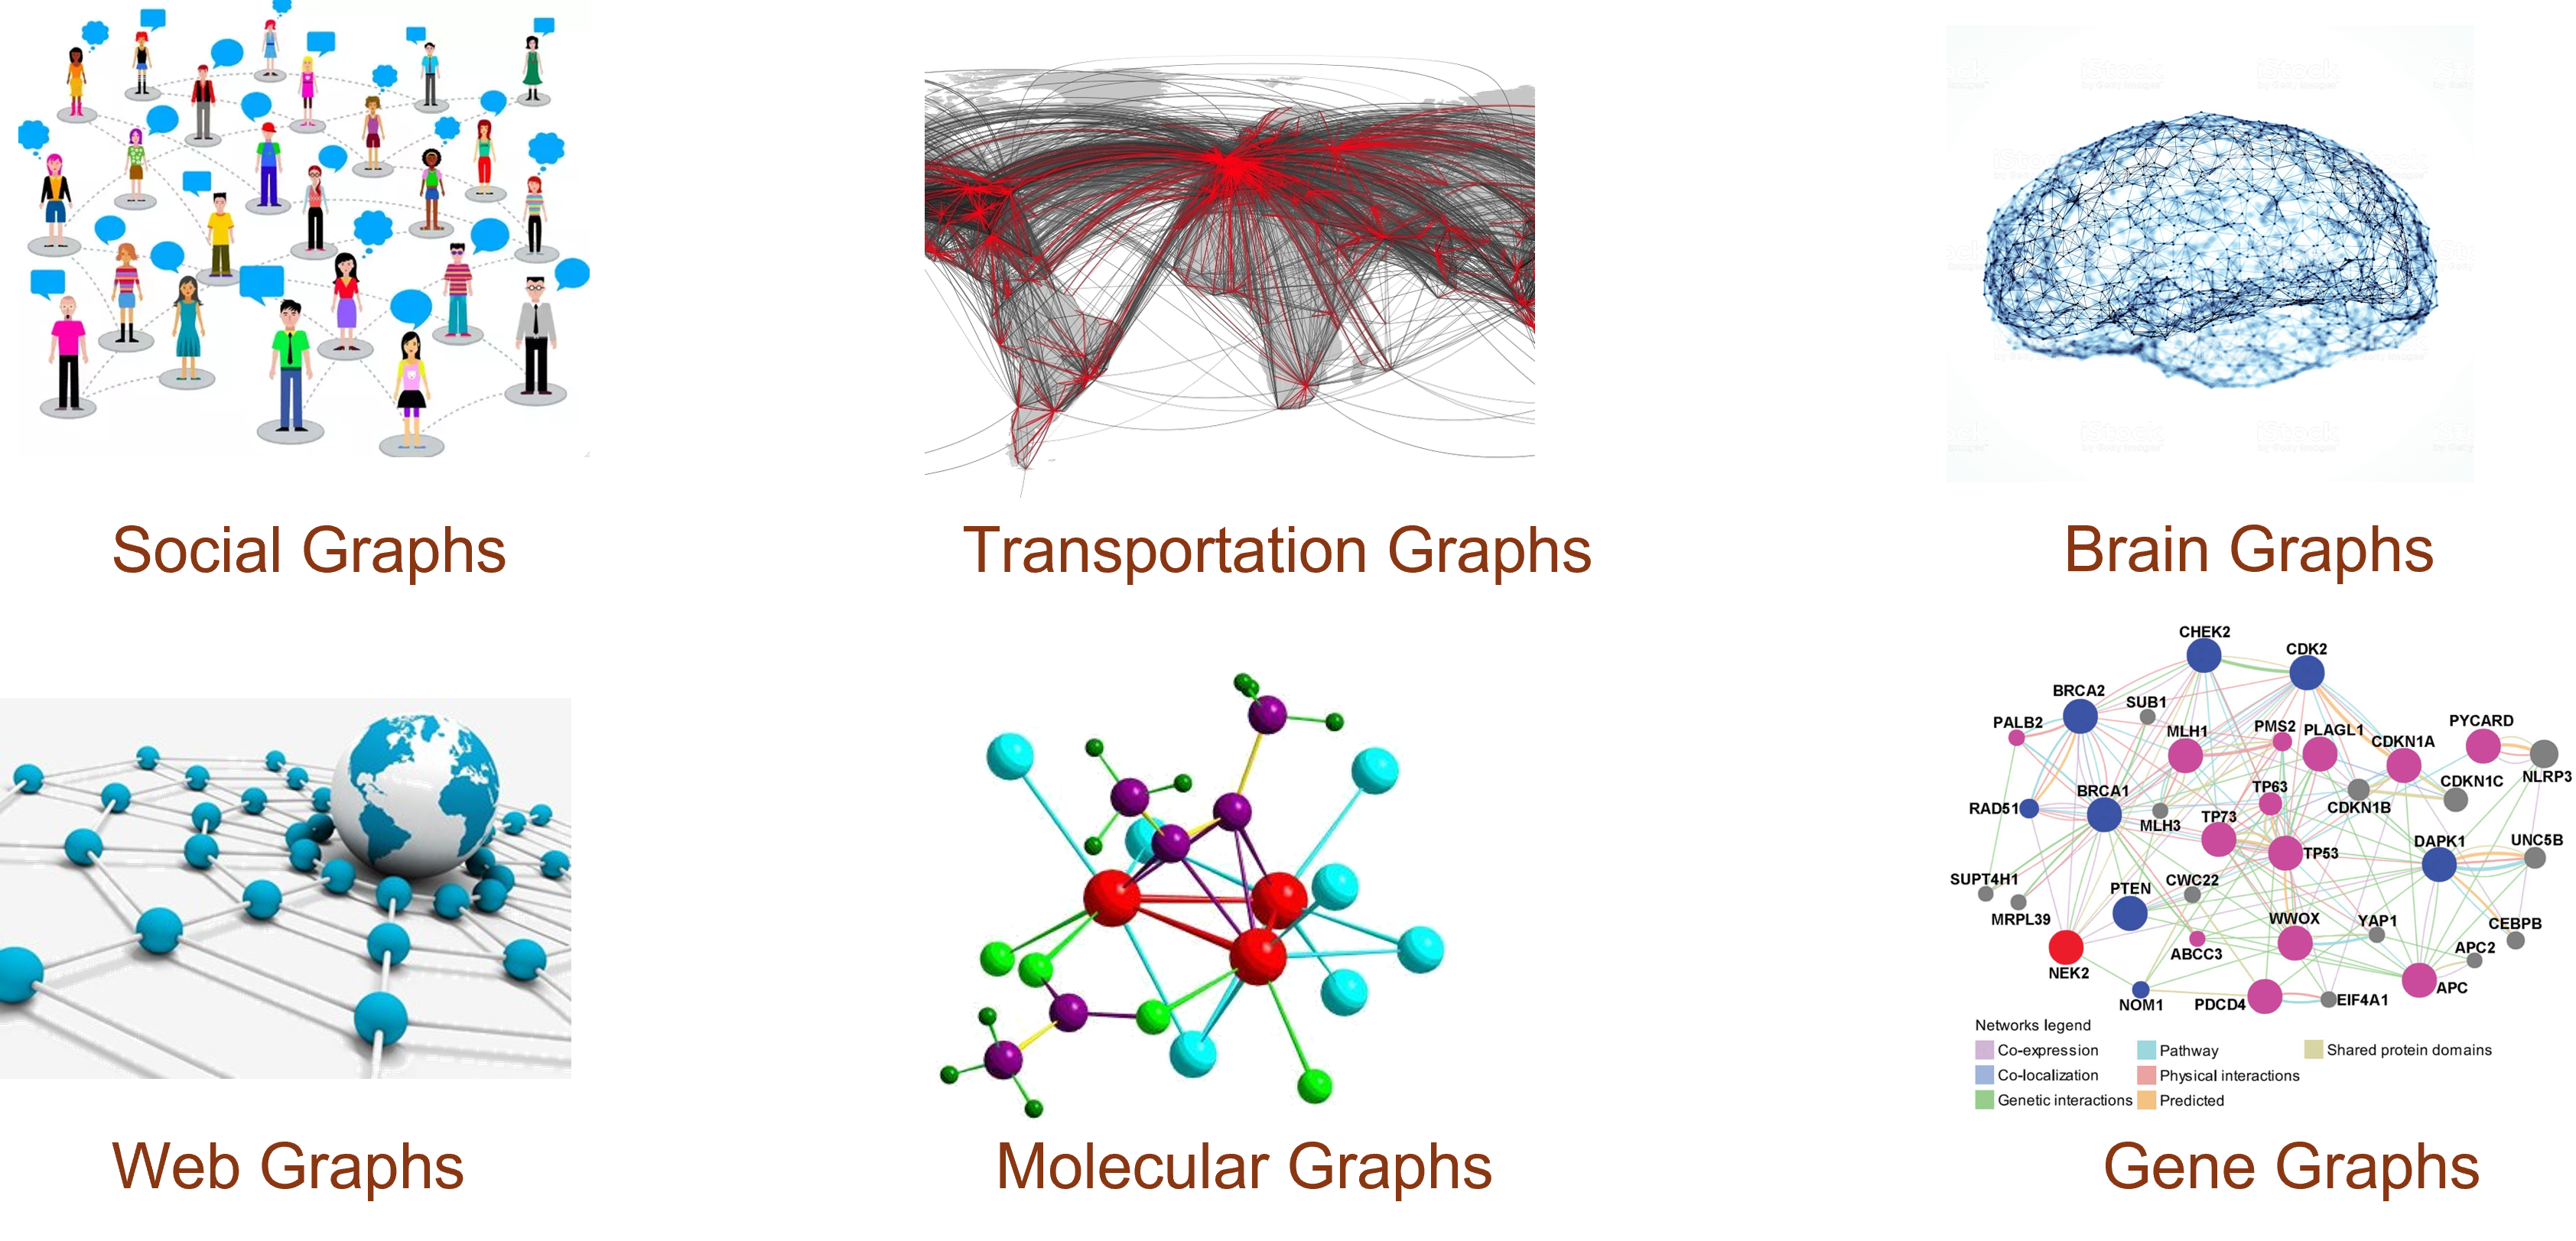
\includegraphics[width=\linewidth,keepaspectratio]{gnn5}
\end{center}	  

\end{frame}

%%%%%%%%%%%%%%%%%%%%%%%%%%%%%%%%%%%%%%%%%%%%%%%%%%%%%%%%%%%
\begin{frame}[fragile]\frametitle{Data as Graphs - Implicit }

\begin{center}
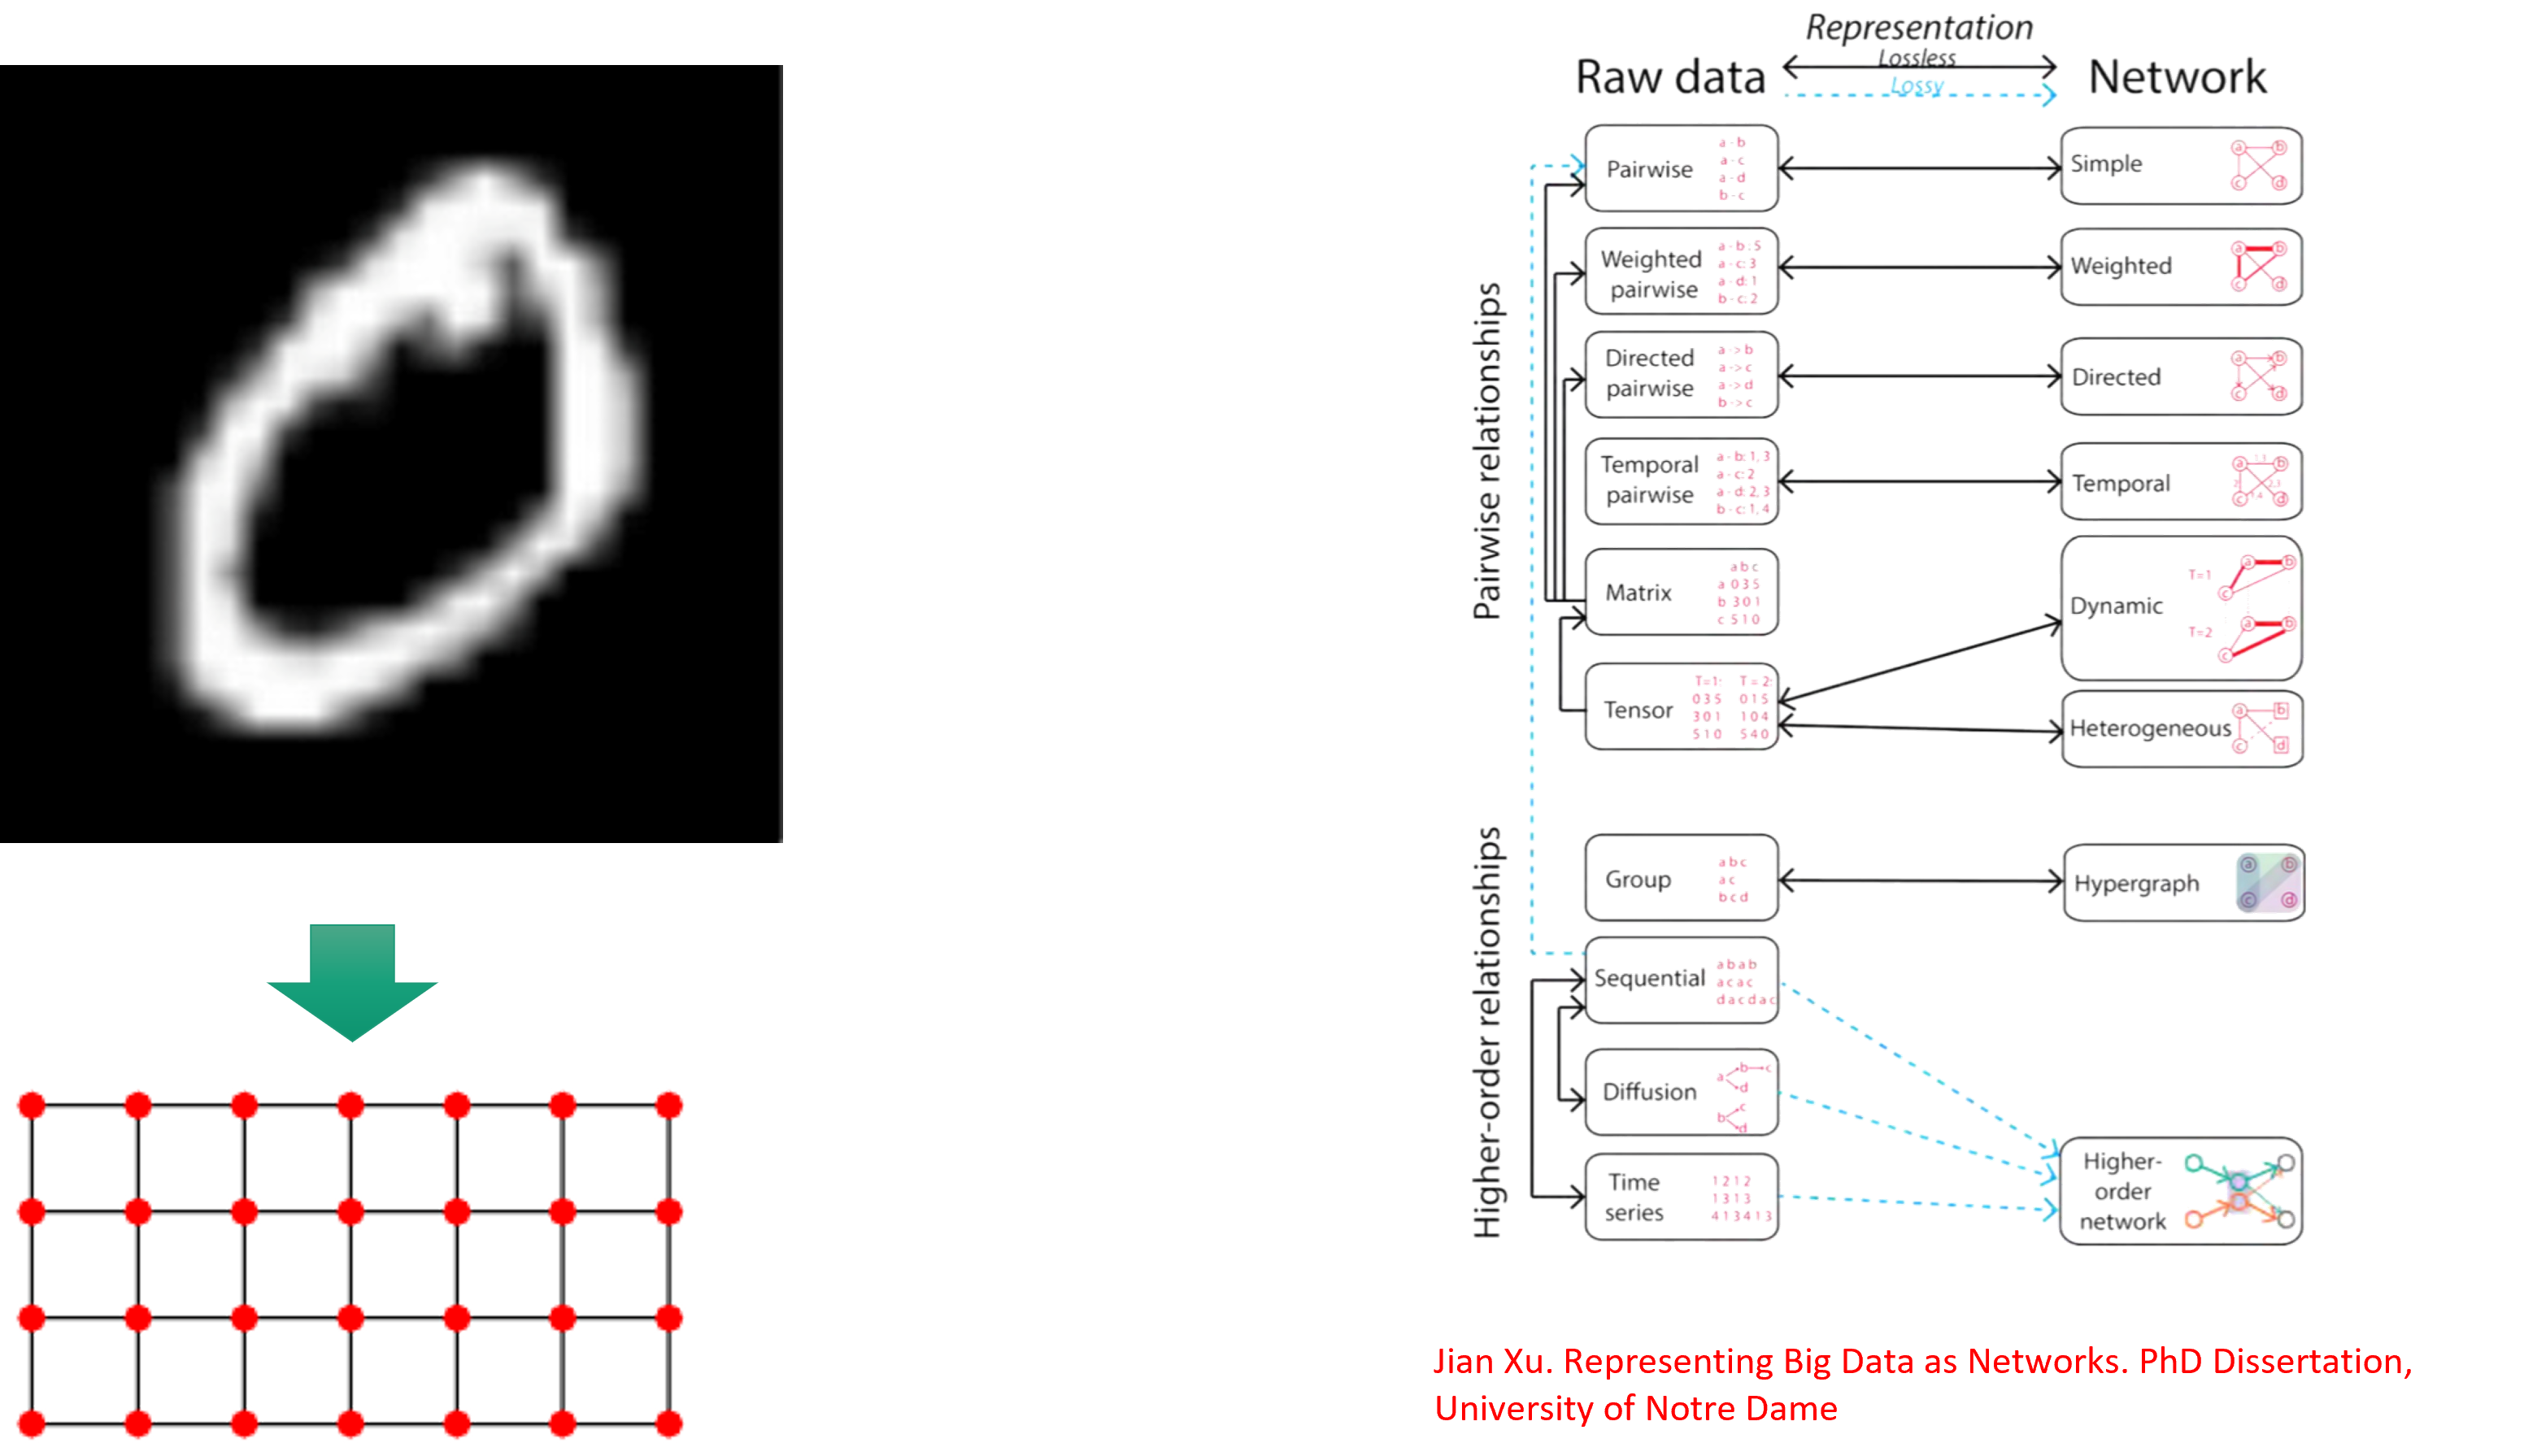
\includegraphics[width=\linewidth,keepaspectratio]{gnn6}
\end{center}	  

\end{frame}



%%%%%%%%%%%%%%%%%%%%%%%%%%%%%%%%%%%%%%%%%%%%%%%%%%%%%%%%%%%
\begin{frame}[fragile]\frametitle{}

\begin{center}
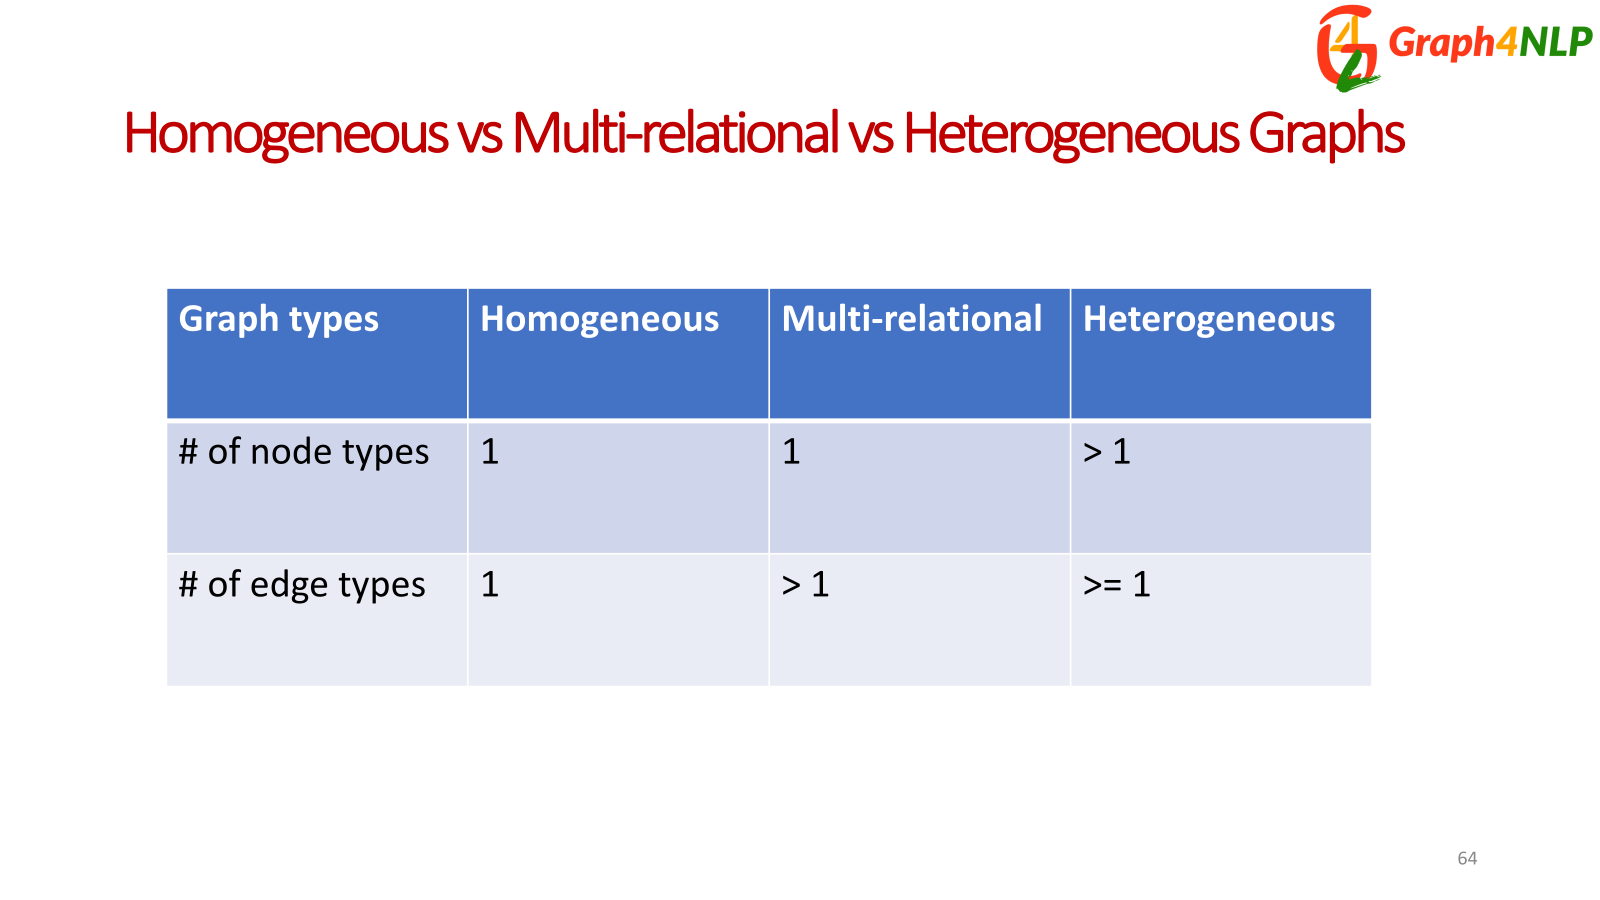
\includegraphics[width=\linewidth,keepaspectratio]{gnn8}
\end{center}	  

\end{frame}


%%%%%%%%%%%%%%%%%%%%%%%%%%%%%%%%%%%%%%%%%%%%%%%%%%%%%%%%%%%%%%%%%%%%%%%%%%%%%%%%%%
\begin{frame}\frametitle{Graph Components}

\begin{itemize}
\item Node (Vertex): A must data element for constructing a graph
\item Relationship (Edge) : Link between two nodes, can have direction and type.
\item Label: Node category/type such as PERSON, ORG, etc. One node can have many types.
\item Properties: Attributes or fields in Nodes or Edges, eg. A node can have Label PERSON and Property such as ``name: Jane''
\end{itemize}



{\tiny (Ref: Introduction to Neo4j - a hands-on crash course - neo4j)}
\end{frame}




%%%%%%%%%%%%%%%%%%%%%%%%%%%%%%%%%%%%%%%%%%%%%%%%%%%%%%%%%%%%%%%%%%%%%%%%%%%%%%%%%%
\begin{frame}\frametitle{Nodes}


\begin{center}
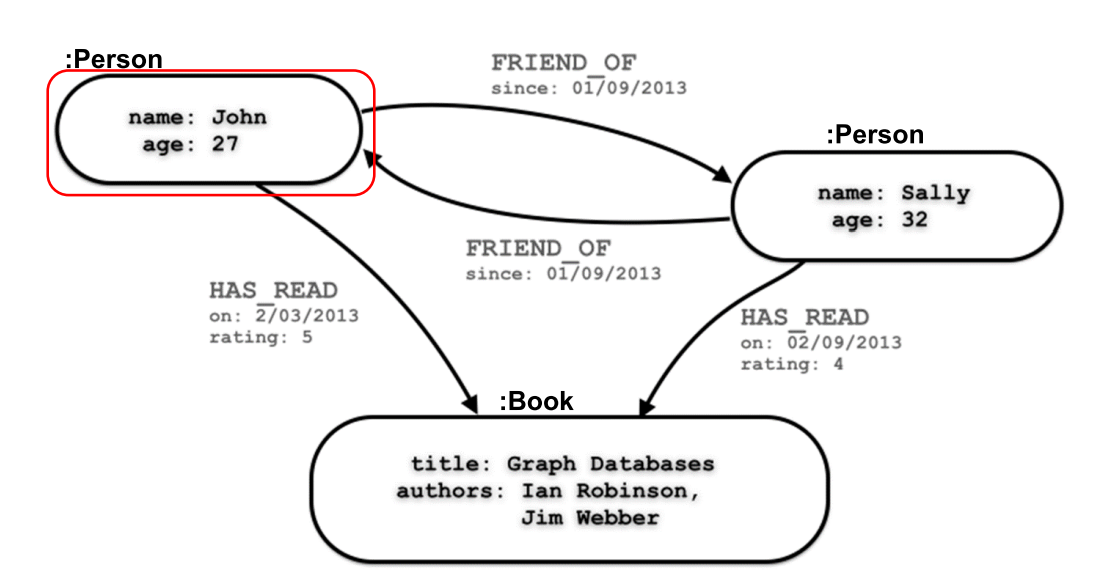
\includegraphics[width=\linewidth,keepaspectratio]{neo4j33}
\end{center}	

{\tiny (Ref: CIS 6930 - Advanced Databases - Neo4j )}
\end{frame}


%%%%%%%%%%%%%%%%%%%%%%%%%%%%%%%%%%%%%%%%%%%%%%%%%%%%%%%%%%%%%%%%%%%%%%%%%%%%%%%%%%
\begin{frame}\frametitle{Relationships}


\begin{center}
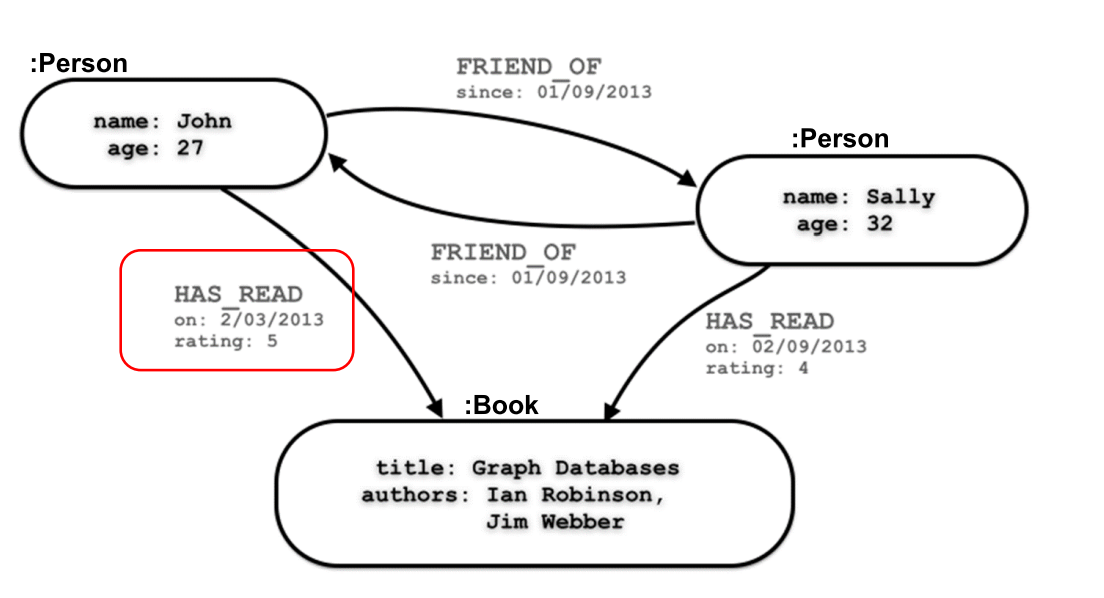
\includegraphics[width=\linewidth,keepaspectratio]{neo4j34}
\end{center}	

{\tiny (Ref: CIS 6930 - Advanced Databases - Neo4j )}
\end{frame}

%%%%%%%%%%%%%%%%%%%%%%%%%%%%%%%%%%%%%%%%%%%%%%%%%%%%%%%%%%%%%%%%%%%%%%%%%%%%%%%%%%
\begin{frame}\frametitle{Properties}


\begin{center}
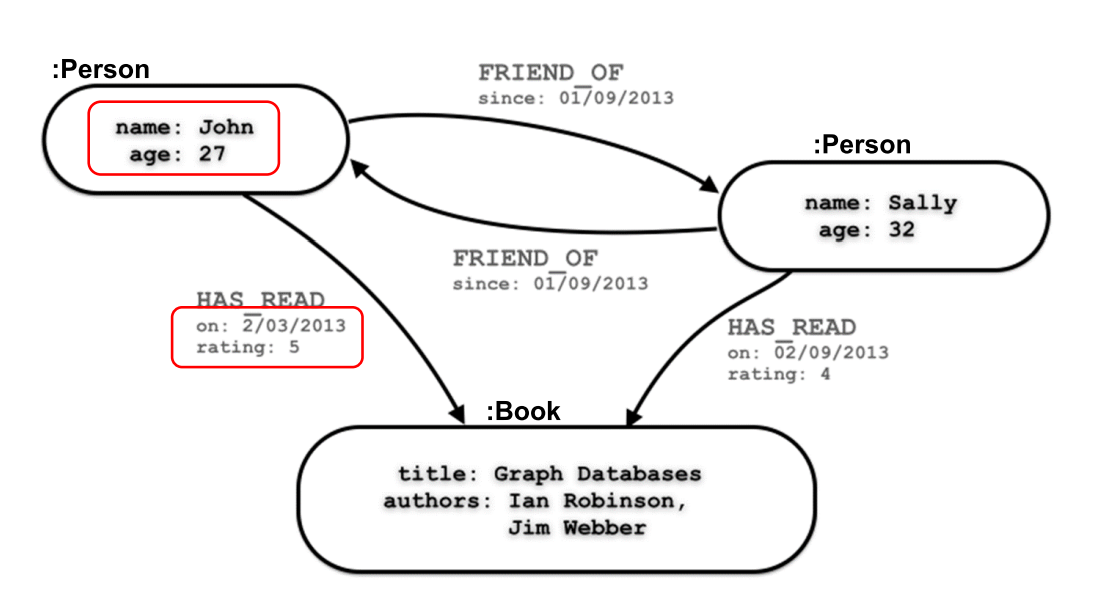
\includegraphics[width=\linewidth,keepaspectratio]{neo4j35}
\end{center}	

{\tiny (Ref: CIS 6930 - Advanced Databases - Neo4j )}
\end{frame}


%%%%%%%%%%%%%%%%%%%%%%%%%%%%%%%%%%%%%%%%%%%%%%%%%%%%%%%%%%%%%%%%%%%%%%%%%%%%%%%%%%
\begin{frame}\frametitle{Labels}


\begin{center}
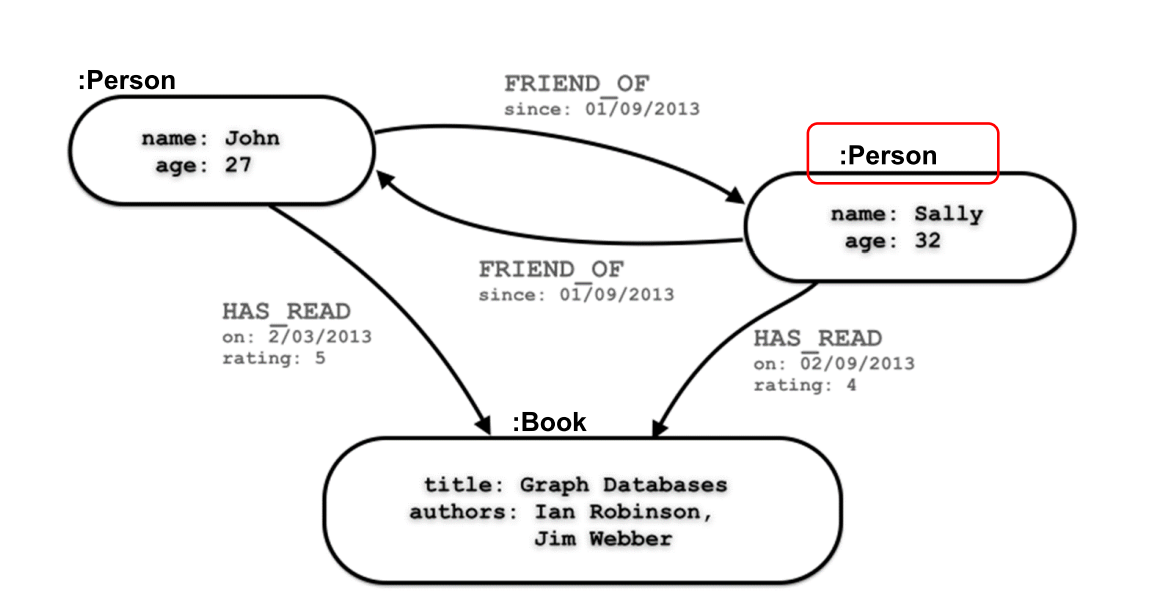
\includegraphics[width=\linewidth,keepaspectratio]{neo4j36}
\end{center}	

{\tiny (Ref: CIS 6930 - Advanced Databases - Neo4j )}
\end{frame}


%%%%%%%%%%%%%%%%%%%%%%%%%%%%%%%%%%%%%%%%%%%%%%%%%%%%%%%%%%%%%%%%%%%%%%%%%%%%%%%%%%
\begin{frame}\frametitle{Graph-Edge Types}

\begin{itemize}
\item Undirected graph: edges are bidirectional, e.g. Michale is brother of John, necessarily means that John is brother of Michale.
\item Directed graph: edges have one direction, e.g. A likes B does not necessarily mean that B likes A.
\item Weighted graph: edges have weights, e.g. connection from city A to city B via road R1 will have wright, say, 8, due to high traffic, but via road R2, may have weight 2, due to lower traffic.
\end{itemize}

\end{frame}

%%%%%%%%%%%%%%%%%%%%%%%%%%%%%%%%%%%%%%%%%%%%%%%%%%%%%%%%%%%%%%%%%%%%%%%%%%%%%%%%%%
\begin{frame}\frametitle{Shortest Path}

\begin{itemize}
\item Find shortest path in a weighted graph, to save logistic costs
\item Dijkstra's or A* algorithm
\item Graph Traversals: can edges be traversed multiple times or nodes traversed multiple times? Neo4j prefers not to traverse edges multiple times, thus making it fast.
\end{itemize}

Application: :
\begin{center}
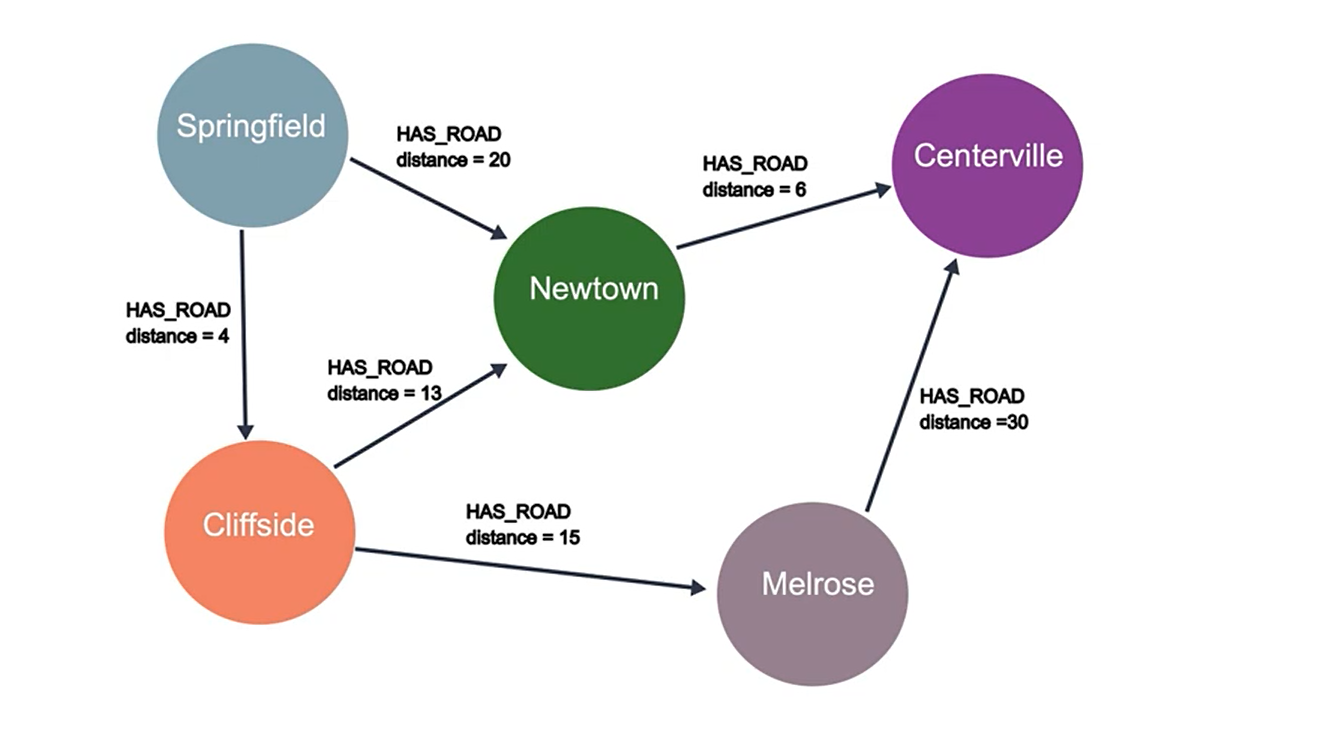
\includegraphics[width=0.6\linewidth,keepaspectratio]{neo4j55}
\end{center}	

How many unique paths are there from Springfield to CenterVille?

{\tiny (Ref: Introduction to Neo4j - a hands-on crash course - neo4j)}
\end{frame}

%%%%%%%%%%%%%%%%%%%%%%%%%%%%%%%%%%%%%%%%%%%%%%%%%%%%%%%%%%%%%%%%%%%%%%%%%%%%%%%%%%
\begin{frame}\frametitle{Summary: Different Kinds of Graphs}

\begin{center}
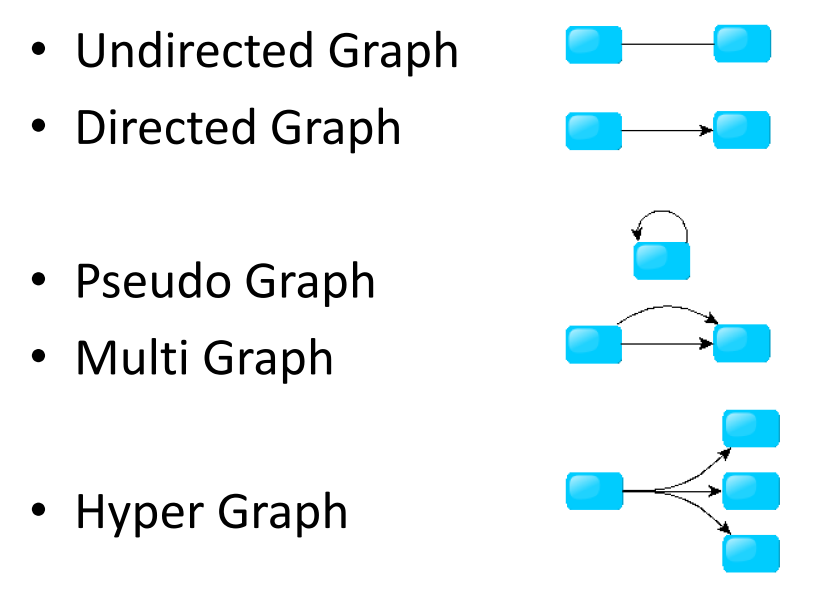
\includegraphics[width=0.5\linewidth,keepaspectratio]{neo4j41}
\end{center}
 

{\tiny (Ref: CIntroduction to Graph Databases - Max De Marzi )}
\end{frame}

%%%%%%%%%%%%%%%%%%%%%%%%%%%%%%%%%%%%%%%%%%%%%%%%%%%%%%%%%%%%%%%%%%%%%%%%%%%%%%%%%%
\begin{frame}\frametitle{Summary: More Kinds of Graphs}

\begin{center}
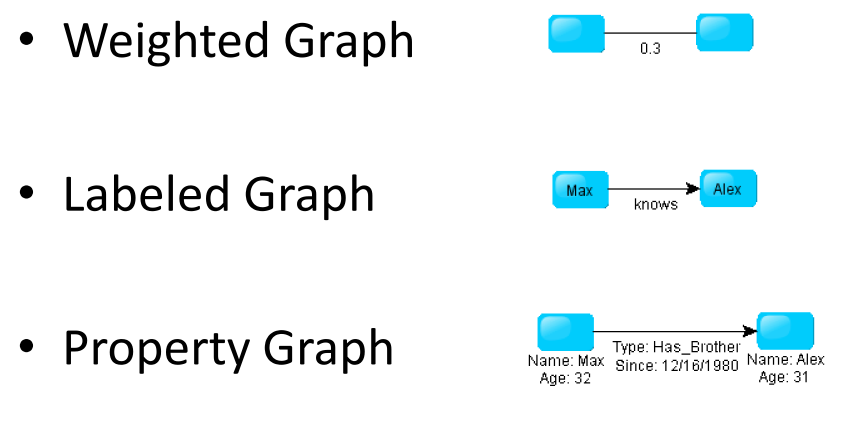
\includegraphics[width=0.5\linewidth,keepaspectratio]{neo4j42}
\end{center}
 

{\tiny (Ref: CIntroduction to Graph Databases - Max De Marzi )}
\end{frame}


%%%%%%%%%%%%%%%%%%%%%%%%%%%%%%%%%%%%%%%%%%%%%%%%%%%%%%%%%%%
\begin{frame}[fragile]\frametitle{Graphs and features}

\begin{center}
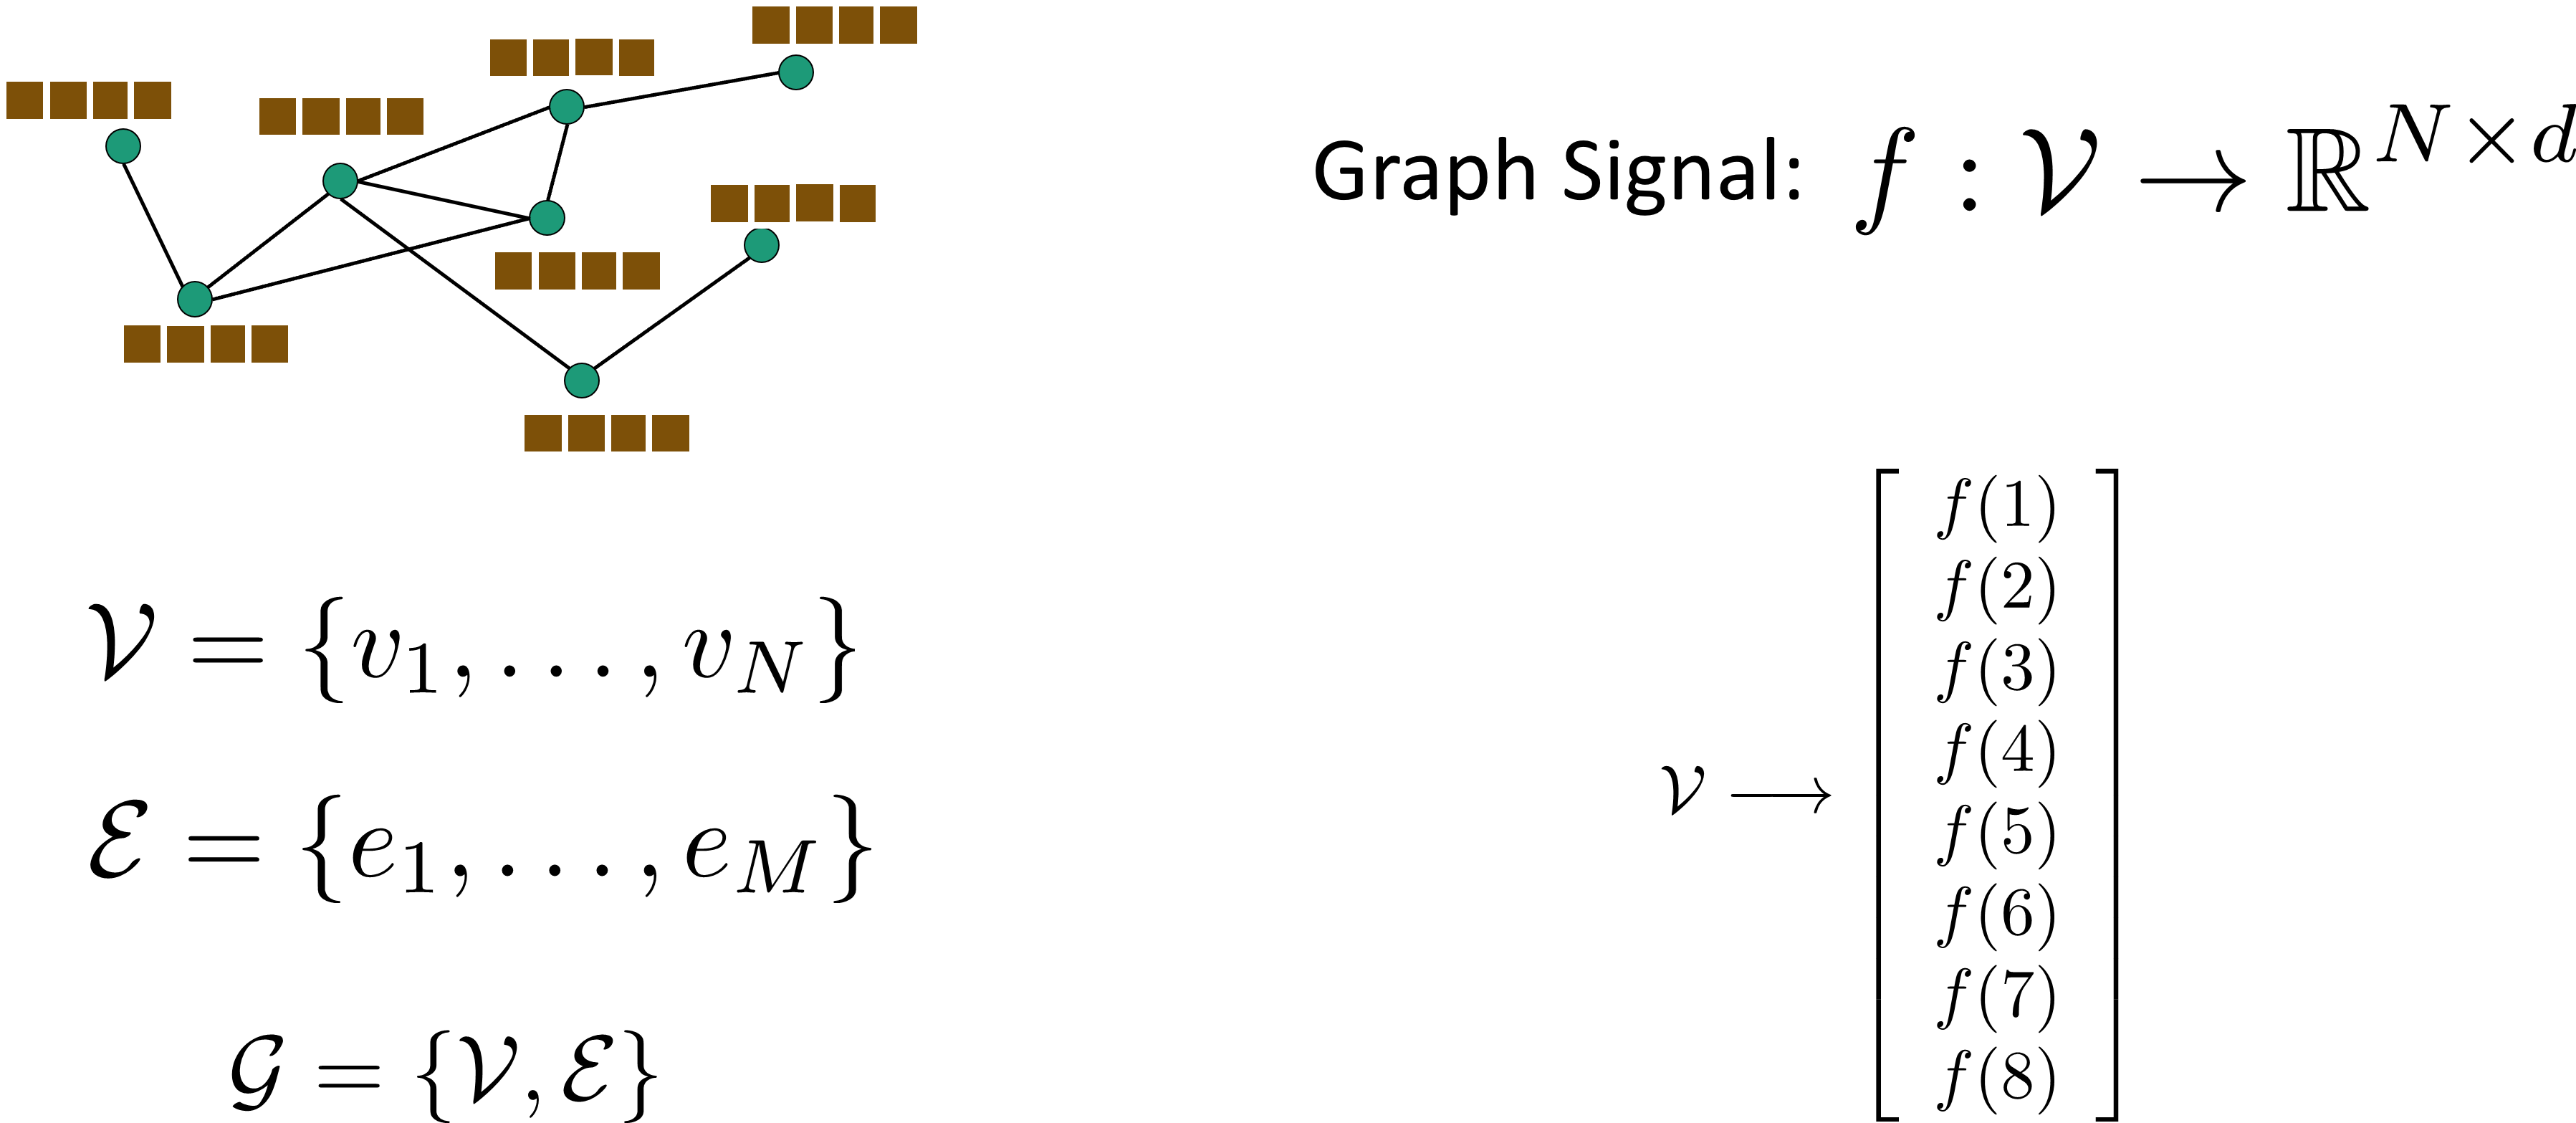
\includegraphics[width=\linewidth,keepaspectratio]{gnn9}
\end{center}	  

\end{frame}

%%%%%%%%%%%%%%%%%%%%%%%%%%%%%%%%%%%%%%%%%%%%%%%%%%%%%%%%%%%
\begin{frame}[fragile]\frametitle{Matrix Representations of Graphs}

\begin{center}
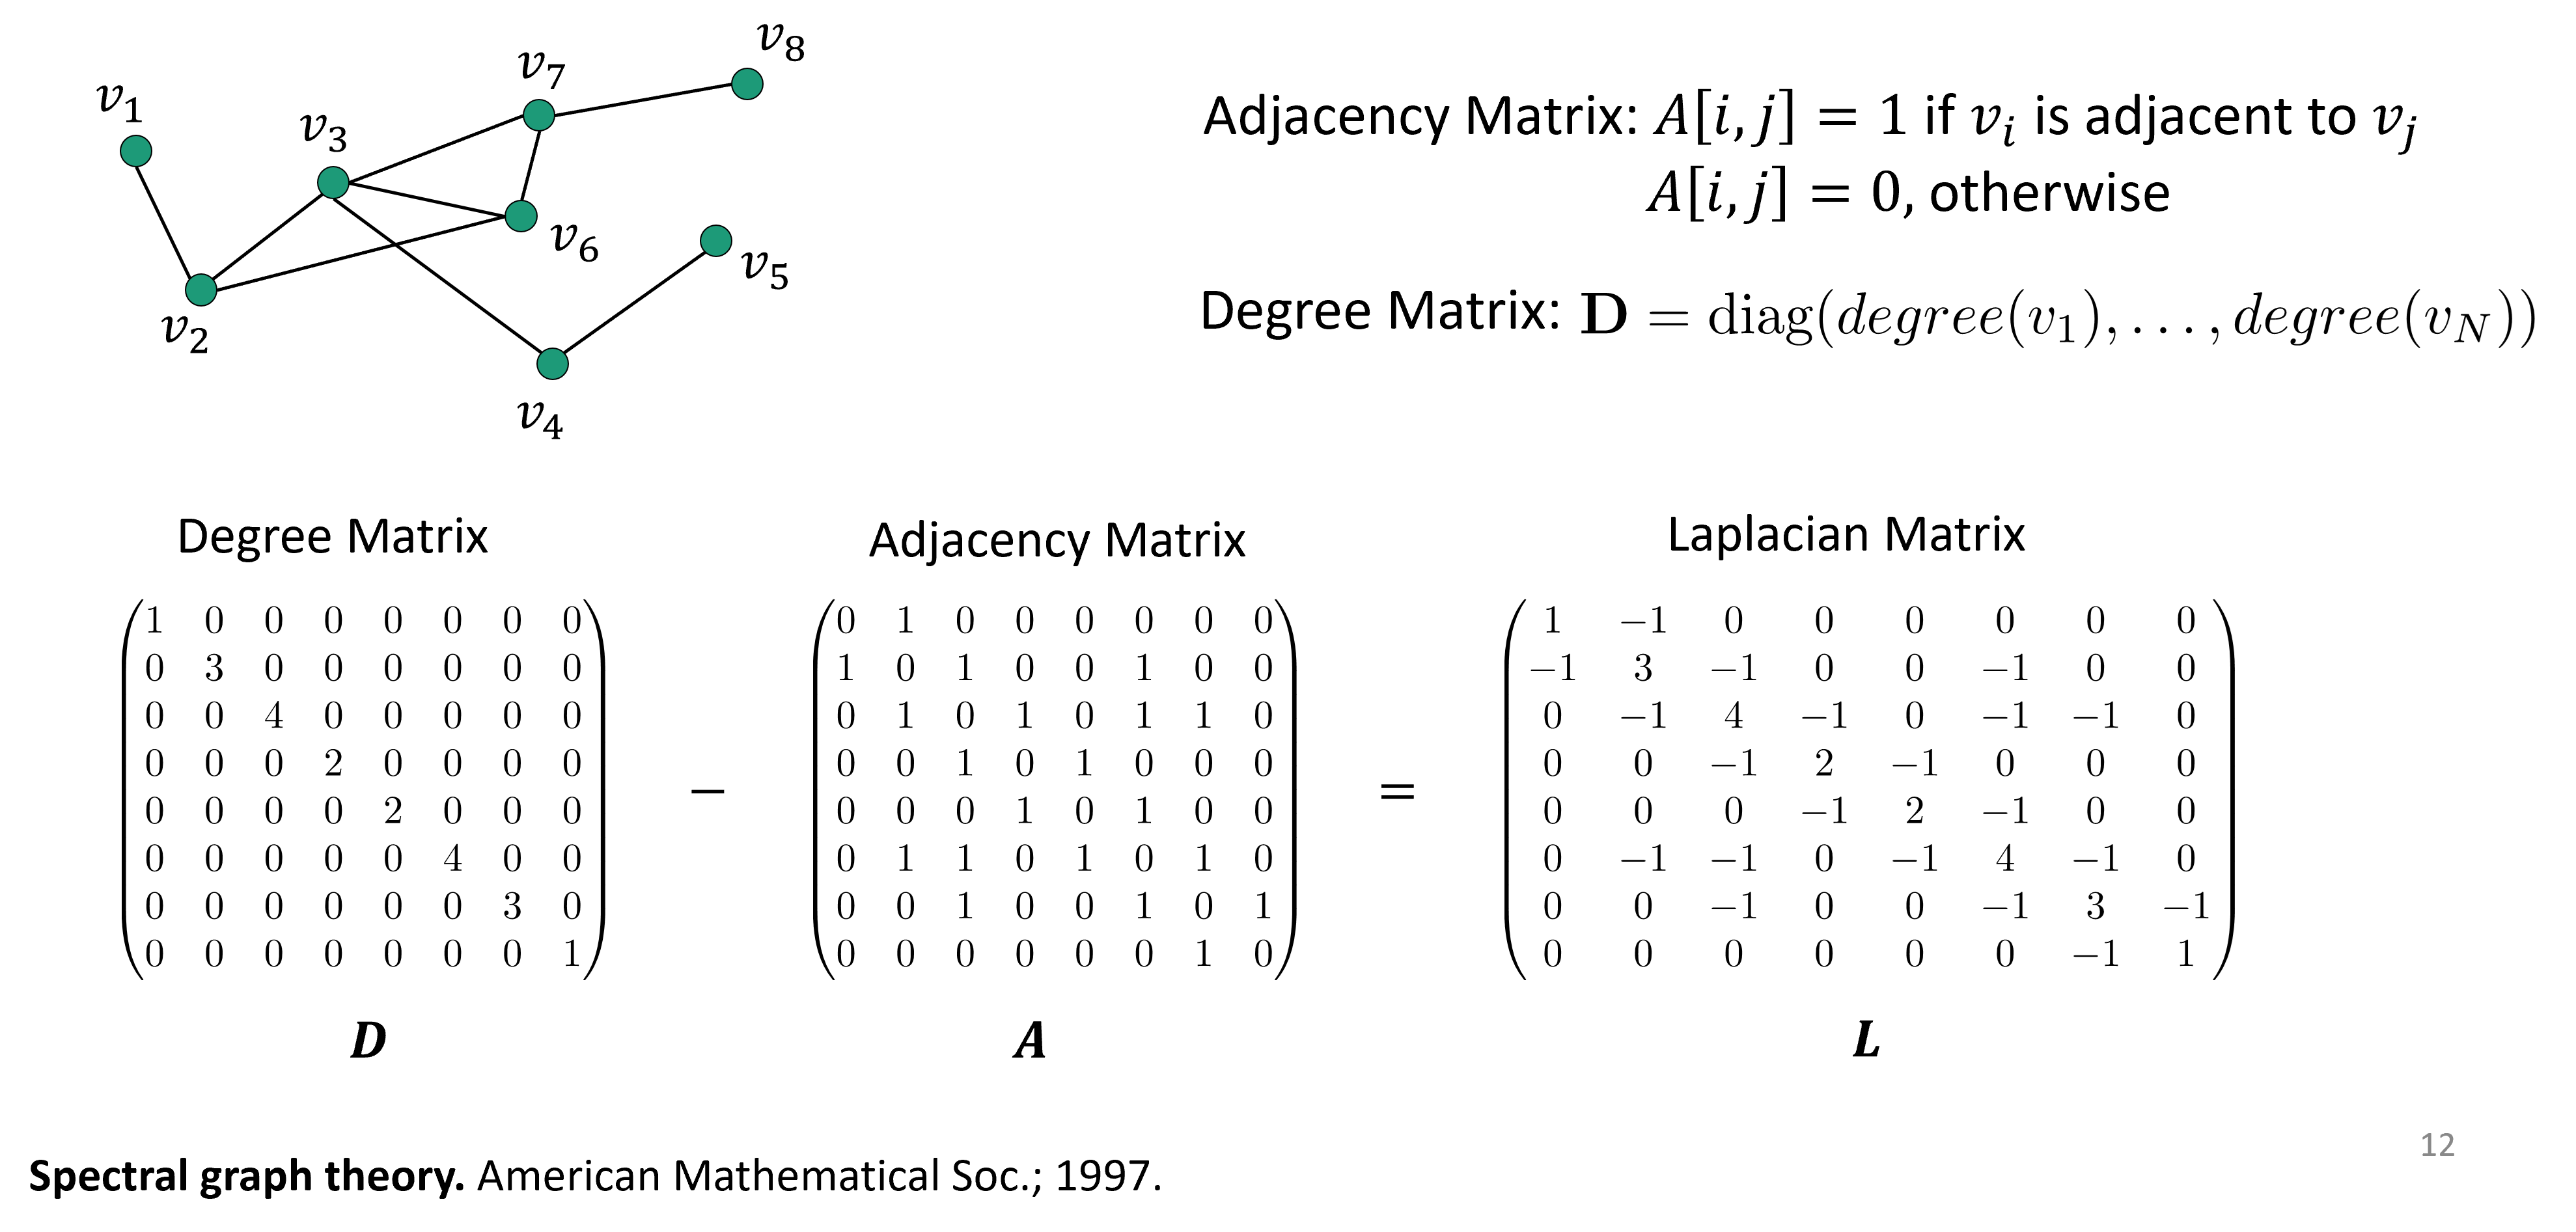
\includegraphics[width=\linewidth,keepaspectratio]{gnn10}
\end{center}	  

\end{frame}


%%%%%%%%%%%%%%%%%%%%%%%%%%%%%%%%%%%%%%%%%%%%%%%%%%%%%%%%%%
\begin{frame}[fragile]\frametitle{Why Graphs? Why Now?}

\begin{itemize}
\item Universal language for describing complex data: Networks/graphs from science, nature, and technology are more similar than one would expect
\item Shared vocabulary between fields: Computer Science, Social science, Physics, Biology, Economics 
\item Data availability (+ computational challenges): Social/Internet, text, logic, program, bio, health, and medical
\item Impact: Social networking, Social media, Drug design, Event detection, Natural language processing, Computer vision, and Logic reasoning
\end{itemize}

\end{frame}

%%%%%%%%%%%%%%%%%%%%%%%%%%%%%%%%%%%%%%%%%%%%%%%%%%%%%%%%%%%%%%%%%%%%%%%%%%%%%%%%%%
\begin{frame}\frametitle{Identifying good Graph scenarios - 1/4}

Does the problem involve understanding relationships between entities?

Behavioral analysis:

\begin{center}
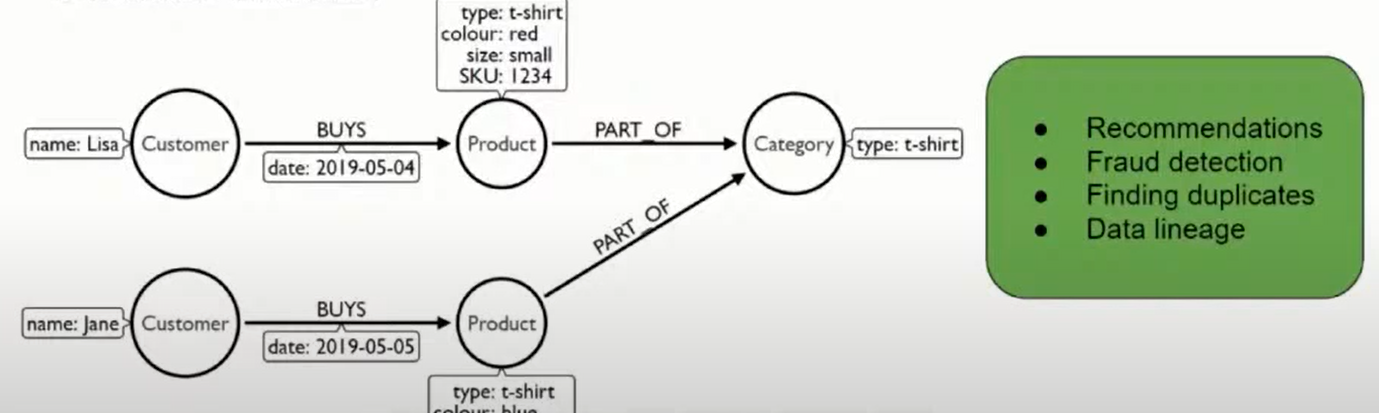
\includegraphics[width=\linewidth,keepaspectratio]{neo4j5}
\end{center}	  

{\tiny (Ref: Introduction to Neo4j - a hands-on crash course - neo4j)}
\end{frame}

%%%%%%%%%%%%%%%%%%%%%%%%%%%%%%%%%%%%%%%%%%%%%%%%%%%%%%%%%%%%%%%%%%%%%%%%%%%%%%%%%%
\begin{frame}\frametitle{Identifying good Graph scenarios - 2/4}

Does the problem involve a lot of self-referencing to the same type of entity?

Org chart of employees:

\begin{center}
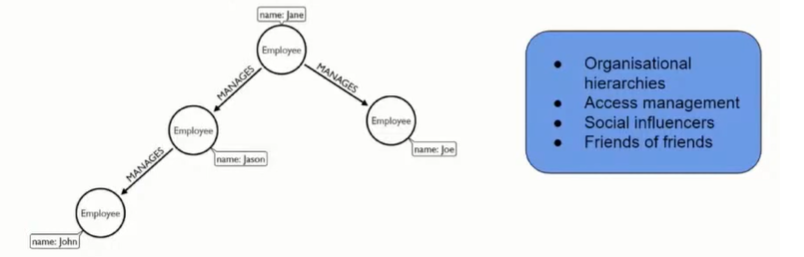
\includegraphics[width=\linewidth,keepaspectratio]{neo4j6}
\end{center}	  

{\tiny (Ref: Introduction to Neo4j - a hands-on crash course - neo4j)}
\end{frame}

%%%%%%%%%%%%%%%%%%%%%%%%%%%%%%%%%%%%%%%%%%%%%%%%%%%%%%%%%%%%%%%%%%%%%%%%%%%%%%%%%%
\begin{frame}\frametitle{Identifying good Graph scenarios - 3/4}

Does the problem explore relationships of varying and unknown depth?

Changes in manufacturing process:

\begin{center}
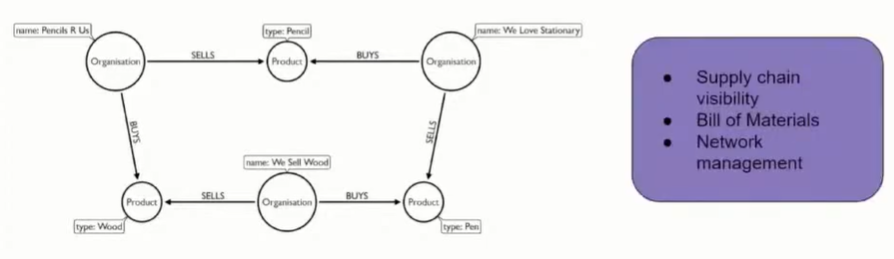
\includegraphics[width=\linewidth,keepaspectratio]{neo4j7}
\end{center}	  

{\tiny (Ref: Introduction to Neo4j - a hands-on crash course - neo4j)}
\end{frame}

%%%%%%%%%%%%%%%%%%%%%%%%%%%%%%%%%%%%%%%%%%%%%%%%%%%%%%%%%%%%%%%%%%%%%%%%%%%%%%%%%%
\begin{frame}\frametitle{Identifying good Graph scenarios - 4/4}

Does the problem involve discovering lots of different routes or paths?

Optimum logistics:

\begin{center}
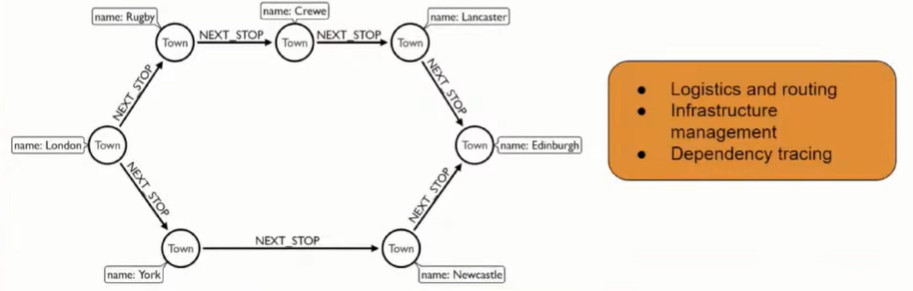
\includegraphics[width=\linewidth,keepaspectratio]{neo4j8}
\end{center}	  

{\tiny (Ref: Introduction to Neo4j - a hands-on crash course - neo4j)}
\end{frame}

%%%%%%%%%%%%%%%%%%%%%%%%%%%%%%%%%%%%%%%%%%%%%%%%%%%%%%%%%%%%%%%%%%%%%%%%%%%%%%%%%%
\begin{frame}\frametitle{Common Use cases: E-Commerce Recommendations}


Easy in graph databases: those who bought A also bought B.

\begin{center}
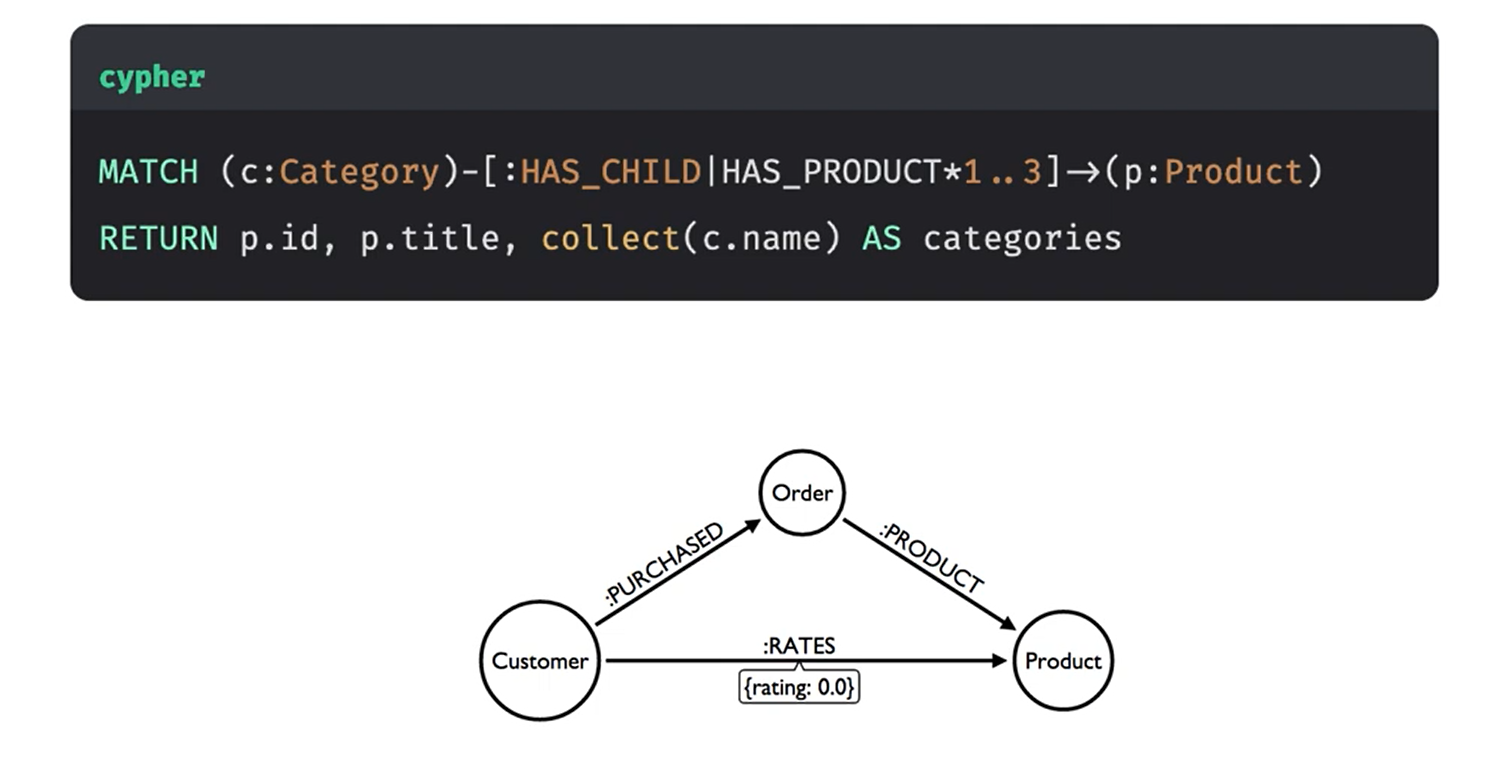
\includegraphics[width=\linewidth,keepaspectratio]{neo4j56}
\end{center}	

{\tiny (Ref: Introduction to Neo4j - a hands-on crash course - neo4j)}
\end{frame}

%%%%%%%%%%%%%%%%%%%%%%%%%%%%%%%%%%%%%%%%%%%%%%%%%%%%%%%%%%%%%%%%%%%%%%%%%%%%%%%%%%
\begin{frame}\frametitle{Common Use cases: Investigative Journalism}

Panama papers: Identify corruption based on relationships between people/companies/financial-institutions.

\begin{center}
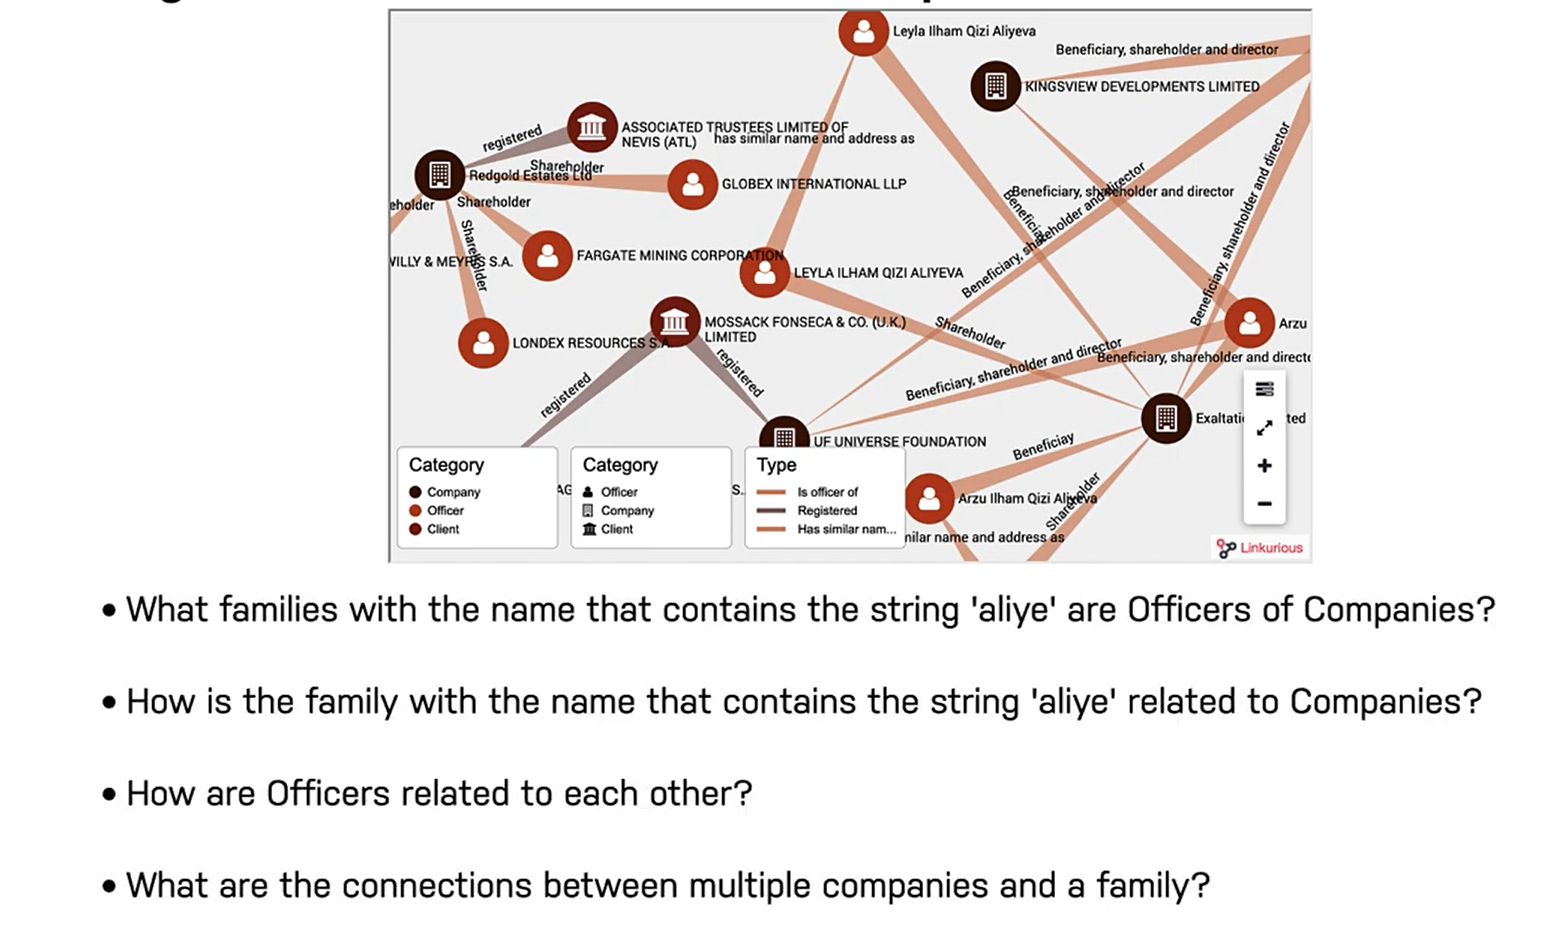
\includegraphics[width=0.8\linewidth,keepaspectratio]{neo4j57}
\end{center}	

{\tiny (Ref: Introduction to Neo4j - a hands-on crash course - neo4j)}
\end{frame}

%%%%%%%%%%%%%%%%%%%%%%%%%%%%%%%%%%%%%%%%%%%%%%%%%%%%%%%%%%%%%%%%%%%%%%%%%%%%%%%%%%
\begin{frame}\frametitle{Common Use cases: Network Dependencies}



\begin{center}
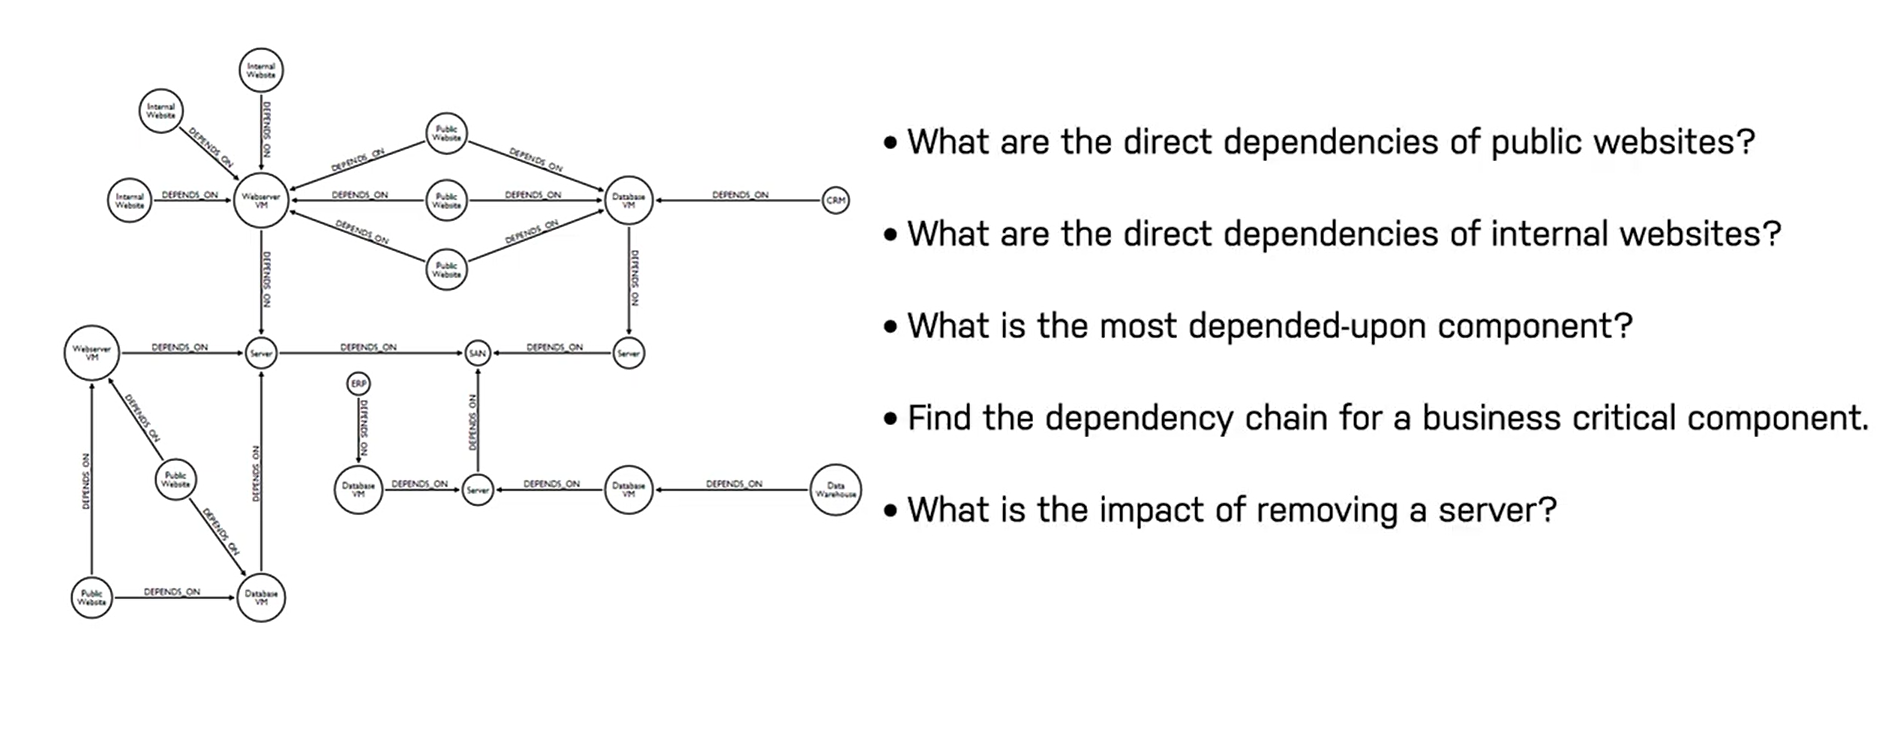
\includegraphics[width=\linewidth,keepaspectratio]{neo4j58}
\end{center}	

{\tiny (Ref: Introduction to Neo4j - a hands-on crash course - neo4j)}
\end{frame}


%%%%%%%%%%%%%%%%%%%%%%%%%%%%%%%%%%%%%%%%%%%%%%%%%%%%%%%%%%%%%%%%%%%%%%%%%%%%%%%%%%
\begin{frame}\frametitle{Common Use cases: Supply Chain}



\begin{center}
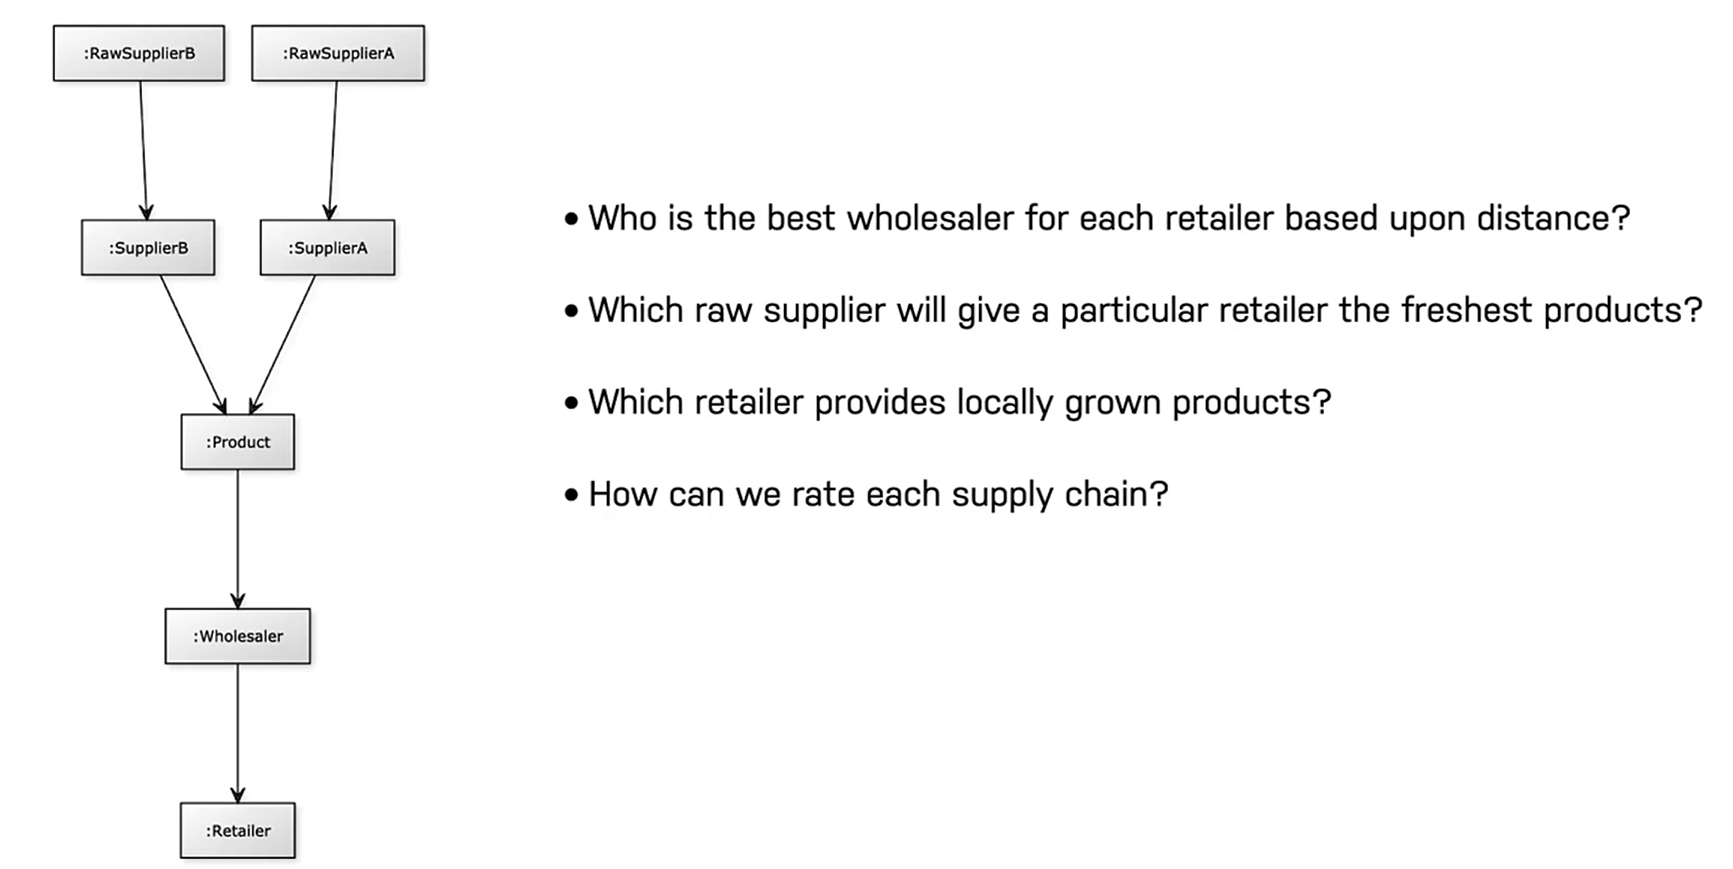
\includegraphics[width=\linewidth,keepaspectratio]{neo4j59}
\end{center}	

{\tiny (Ref: Introduction to Neo4j - a hands-on crash course - neo4j)}
\end{frame}

